\documentclass{article}\usepackage[]{graphicx}\usepackage[]{color}
% maxwidth is the original width if it is less than linewidth
% otherwise use linewidth (to make sure the graphics do not exceed the margin)
\makeatletter
\def\maxwidth{ %
  \ifdim\Gin@nat@width>\linewidth
    \linewidth
  \else
    \Gin@nat@width
  \fi
}
\makeatother

\definecolor{fgcolor}{rgb}{0.345, 0.345, 0.345}
\newcommand{\hlnum}[1]{\textcolor[rgb]{0.686,0.059,0.569}{#1}}%
\newcommand{\hlstr}[1]{\textcolor[rgb]{0.192,0.494,0.8}{#1}}%
\newcommand{\hlcom}[1]{\textcolor[rgb]{0.678,0.584,0.686}{\textit{#1}}}%
\newcommand{\hlopt}[1]{\textcolor[rgb]{0,0,0}{#1}}%
\newcommand{\hlstd}[1]{\textcolor[rgb]{0.345,0.345,0.345}{#1}}%
\newcommand{\hlkwa}[1]{\textcolor[rgb]{0.161,0.373,0.58}{\textbf{#1}}}%
\newcommand{\hlkwb}[1]{\textcolor[rgb]{0.69,0.353,0.396}{#1}}%
\newcommand{\hlkwc}[1]{\textcolor[rgb]{0.333,0.667,0.333}{#1}}%
\newcommand{\hlkwd}[1]{\textcolor[rgb]{0.737,0.353,0.396}{\textbf{#1}}}%
\let\hlipl\hlkwb

\usepackage{framed}
\makeatletter
\newenvironment{kframe}{%
 \def\at@end@of@kframe{}%
 \ifinner\ifhmode%
  \def\at@end@of@kframe{\end{minipage}}%
  \begin{minipage}{\columnwidth}%
 \fi\fi%
 \def\FrameCommand##1{\hskip\@totalleftmargin \hskip-\fboxsep
 \colorbox{shadecolor}{##1}\hskip-\fboxsep
     % There is no \\@totalrightmargin, so:
     \hskip-\linewidth \hskip-\@totalleftmargin \hskip\columnwidth}%
 \MakeFramed {\advance\hsize-\width
   \@totalleftmargin\z@ \linewidth\hsize
   \@setminipage}}%
 {\par\unskip\endMakeFramed%
 \at@end@of@kframe}
\makeatother

\definecolor{shadecolor}{rgb}{.97, .97, .97}
\definecolor{messagecolor}{rgb}{0, 0, 0}
\definecolor{warningcolor}{rgb}{1, 0, 1}
\definecolor{errorcolor}{rgb}{1, 0, 0}
\newenvironment{knitrout}{}{} % an empty environment to be redefined in TeX

\usepackage{alltt}
\usepackage{amsmath} %This allows me to use the align functionality.
                     %If you find yourself trying to replicate
                     %something you found online, ensure you're
                     %loading the necessary packages!
\usepackage{amsfonts}%Math font
\usepackage{graphicx}%For including graphics
\usepackage{hyperref}%For Hyperlinks
\hypersetup{colorlinks = true,citecolor=black}
\usepackage{natbib}        %For the bibliography
\bibliographystyle{apalike}%For the bibliography
\usepackage[margin=0.75in]{geometry}
\usepackage{float}
\IfFileExists{upquote.sty}{\usepackage{upquote}}{}
\begin{document}
\noindent \textbf{MA 354: Data Analysis I -- Fall 2021}\\%\\ gives you a new line
\noindent \textbf{Homework 4:}\vspace{1em}\\
\emph{Complete the following opportunities to use what we've talked about in class. 
These questions will be graded for correctness, communication and succinctness. 
Ensure you show your work and explain your logic in a legible and refined submission.}
%Comments -- anything after % is not put into the PDF
\begin{enumerate}
%%%%%%%%%%%%%%%%%%%%%%%%%%%%%%%%%%%%%%%%%%%%%%%%%%%%%%%%%%%%%%%%%%%%%%%%%%%%%%%
%%%%%%%%%%%%%%%%%%%%%%%%%%%%%%%%%%%%%%%%%%%%%%%%%%%%%%%%%%%%%%%%%%%%%%%%%%%%%%%
%%%%%%%%%  Question 0
%%%%%%%%%%%%%%%%%%%%%%%%%%%%%%%%%%%%%%%%%%%%%%%%%%%%%%%%%%%%%%%%%%%%%%%%%%%%%%%
%%%%%%%%%%%%%%%%%%%%%%%%%%%%%%%%%%%%%%%%%%%%%%%%%%%%%%%%%%%%%%%%%%%%%%%%%%%%%%%
\item[0.] \textbf{Complete weekly diagnostics.}
  
%%%%%%%%%%%%%%%%%%%%%%%%%%%%%%%%%%%%%%%%%%%%%%%%%%%%%%%%%%%%%%%%%%%%%%%%%%%%%%%
%%%%%%%%%%%%%%%%%%%%%%%%%%%%%%%%%%%%%%%%%%%%%%%%%%%%%%%%%%%%%%%%%%%%%%%%%%%%%%%
%%%%%%%%%  Question 1
%%%%%%%%%%%%%%%%%%%%%%%%%%%%%%%%%%%%%%%%%%%%%%%%%%%%%%%%%%%%%%%%%%%%%%%%%%%%%%%
%%%%%%%%%%%%%%%%%%%%%%%%%%%%%%%%%%%%%%%%%%%%%%%%%%%%%%%%%%%%%%%%%%%%%%%%%%%%%%%
\item On its website, Ozempic, a medication for lowering the risk of major cardiovascular 
events (e.g., heart attack, stroke, etc.), states that 
\begin{itemize}
  \item 66\% of people taking 0.5 mg Ozempic
  \item 73\% of people taking 1 mg Ozempic
  \item 40\% of people taking 100 mg Januvia
\end{itemize}
reached an A1C under 7\%, noting higher A1C is indicative of higher risk of heart disease.

\begin{enumerate}
\item Explain why this statement alone isn't enough to conclude whether there is a statistically 
significant difference among the treatments.\\

If we want to assess the statistically significant difference among the treatments, a t-sample proprotion test would be out best option. However, we don't have quite enough information to run it, since we have only the percents on our hands. We'd require more information (sample size, for example) before we can make any conclusions.

\item The statement on Ozempic's website comes from a phase 3a randomized double-blind study. 
\cite{Ahren17} reports that 409 received Ozempic (0.5 mg), 409 received Ozempic (1 mg), and 407 
received Januvia (100 mg). 
\begin{enumerate}
  \item Determine whether there is sufficient evidence of a difference in rates of attaining an 
  A1C under 7\% across treatments.\\
  
  Now, when we have more information about the treatments, we can use t-sample proportion test. However, before we do that, it would be highly advisable to check the assumptions first.\\
  — Data is representative: check.
  — Two possible outcomes (lowered/did not lower): check.
  — There are more than 10 instances of success and failure: check.
  \begin{align*}
H_{0}&:\hat{p}_{1}=\hat{p}_{2}=\hat{p}_3\\
H_{a}&:\hat{p}_{1}\neq\hat{p}_{2}\neq\hat{p}_{3}\\
\end{align*}
\begin{knitrout}
\definecolor{shadecolor}{rgb}{0.969, 0.969, 0.969}\color{fgcolor}\begin{kframe}
\begin{alltt}
\hlcom{# Successfu/total cases for 0.5 mg Ozempic}
\hlstd{x1} \hlkwb{=} \hlkwd{round}\hlstd{(}\hlnum{0.66}\hlopt{*}\hlnum{409}\hlstd{)}
\hlstd{n1} \hlkwb{=} \hlnum{409}

\hlcom{# Successful/total cases for 1 mg Ozempic}
\hlstd{x2} \hlkwb{=} \hlkwd{round}\hlstd{(}\hlnum{0.73}\hlopt{*}\hlnum{409}\hlstd{)}
\hlstd{n2} \hlkwb{=} \hlnum{409}

\hlcom{# Successful/total cases for 100 mg Januvia}
\hlstd{x3} \hlkwb{=} \hlkwd{round}\hlstd{(}\hlnum{0.4}\hlopt{*}\hlnum{407}\hlstd{)}
\hlstd{n3} \hlkwb{=} \hlnum{407}

\hlstd{answer1}\hlkwb{<-}\hlkwd{prop.test}\hlstd{(}\hlkwc{x} \hlstd{=} \hlkwd{c}\hlstd{(x1, x2, x3),} \hlkwc{n} \hlstd{=} \hlkwd{c}\hlstd{(n1, n2, n3))}
\hlstd{p.value1}\hlkwb{<-}\hlstd{answer1}\hlopt{$}\hlstd{p.value}
\hlstd{decision}\hlkwb{<-}\hlkwd{ifelse}\hlstd{(p.value1}\hlopt{<}\hlnum{0.05}\hlstd{,} \hlstr{"is"}\hlstd{,} \hlstr{"is not"}\hlstd{)}
\hlkwd{paste}\hlstd{(}\hlstr{"The p-value: ("}\hlstd{, p.value1,}\hlstr{")"}\hlstd{,}
      \hlkwc{sep}\hlstd{=}\hlstr{""}\hlstd{)}
\end{alltt}
\begin{verbatim}
## [1] "The p-value: (5.01023071720164e-23)"
\end{verbatim}
\end{kframe}
\end{knitrout}
P-value provides us with statistically significant evidence to reject the null hypothesis in favor of the alternative.

  \item Perform a follow-up analysis for comparing treatments. If you were at high risk for 
  cardiovascular events, which medication would you want to take.
\begin{knitrout}
\definecolor{shadecolor}{rgb}{0.969, 0.969, 0.969}\color{fgcolor}\begin{kframe}
\begin{alltt}
\hlstd{answer2}\hlkwb{<-}\hlkwd{pairwise.prop.test}\hlstd{(}\hlkwc{x} \hlstd{=} \hlkwd{c}\hlstd{(x1, x2, x3),} \hlkwc{n} \hlstd{=} \hlkwd{c}\hlstd{(n1, n2, n3))}
\hlstd{answer2}
\end{alltt}
\begin{verbatim}
## 
## 	Pairwise comparisons using Pairwise comparison of proportions 
## 
## data:  c(x1, x2, x3) out of c(n1, n2, n3) 
## 
##   1       2      
## 2 0.033   -      
## 3 3.6e-13 < 2e-16
## 
## P value adjustment method: holm
\end{verbatim}
\end{kframe}
\end{knitrout}
The closer analysis of the pairwise proportion test provides us with the insight that Ozempic treatment is significantly better than the Januvia treatment (with $p<0.001$). However, when it comes to the differences between Ozempic treatments, it's highly advisable to opt for 0.5mg treatment since it provided statistically better results compared to its 1mg alternative.

\end{enumerate}
\end{enumerate}
\newpage
%%%%%%%%%%%%%%%%%%%%%%%%%%%%%%%%%%%%%%%%%%%%%%%%%%%%%%%%%%%%%%%%%%%%%%%%%%%%%%%
%%%%%%%%%%%%%%%%%%%%%%%%%%%%%%%%%%%%%%%%%%%%%%%%%%%%%%%%%%%%%%%%%%%%%%%%%%%%%%%
%%%%%%%%%  Question 2
%%%%%%%%%%%%%%%%%%%%%%%%%%%%%%%%%%%%%%%%%%%%%%%%%%%%%%%%%%%%%%%%%%%%%%%%%%%%%%%
%%%%%%%%%%%%%%%%%%%%%%%%%%%%%%%%%%%%%%%%%%%%%%%%%%%%%%%%%%%%%%%%%%%%%%%%%%%%%%%
\item Is the ANOVA really robust to Normality? Equal sample size? Equal variance?
To assess this we'll check the ability of ANOVA to detect differences in a 
sample and retain the $\alpha=0.05$ across different settings. This homework 
question was motivated by \cite{Blanca17} who published a simulation study 
about ANOVA.\\

\textbf{Remark:} My professor in graduate school always told me that I didn't
have to memorize any results, I could just derive them. The data analysis
analog to this is that if we have any questions about how a model works
under a given condition (or broken assumption) we can just simulate it!
\begin{enumerate}
  \item Plot the Laplace distribution with $m=0$ and $s=2$; the PDF
  of this distribution is cataloged in \texttt{R} as \texttt{dlaplace()} 
  in the rmutil package, which you'll need to install and load. Superimpose
  the graph of the Gaussian distribution with $\mu=0$ and $\sigma=2$. Comment
  on the differences you see and what you think might happen if the data 
  are Laplace distributed instead of the Gaussian distribution.
\begin{knitrout}
\definecolor{shadecolor}{rgb}{0.969, 0.969, 0.969}\color{fgcolor}\begin{kframe}
\begin{alltt}
\hlkwd{library}\hlstd{(rmutil)}
\hlkwd{library}\hlstd{(tidyverse)}

\hlstd{ggdat} \hlkwb{<-} \hlkwd{data.frame}\hlstd{(}\hlkwc{x}\hlstd{=}\hlkwd{seq}\hlstd{(}\hlopt{-}\hlnum{5}\hlstd{,} \hlnum{5}\hlstd{,} \hlkwc{length.out}\hlstd{=}\hlnum{5000}\hlstd{))}\hlopt
\hlkwd{mutate}\hlstd{(}\hlkwc{f}\hlstd{=}\hlkwd{dlaplace}\hlstd{(x,} \hlkwc{m}\hlstd{=}\hlnum{0}\hlstd{,} \hlkwc{s}\hlstd{=}\hlnum{2}\hlstd{),}
       \hlkwc{f1}\hlstd{=}\hlkwd{dnorm}\hlstd{(x,} \hlkwc{mean}\hlstd{=}\hlnum{0}\hlstd{,} \hlkwc{sd}\hlstd{=}\hlnum{2}\hlstd{))}

\hlcom{#set the legend}
\end{alltt}
\end{kframe}
\end{knitrout}
\begin{figure}[H]
\begin{center}
\begin{knitrout}
\definecolor{shadecolor}{rgb}{0.969, 0.969, 0.969}\color{fgcolor}\begin{kframe}
\begin{alltt}
\hlkwd{ggplot}\hlstd{(ggdat,} \hlkwd{aes}\hlstd{(}\hlkwc{x}\hlstd{=x,} \hlkwc{y}\hlstd{=f))}\hlopt{+}
  \hlkwd{geom_line}\hlstd{(}\hlkwc{color}\hlstd{=}\hlstr{"blue"}\hlstd{)}\hlopt{+}
  \hlkwd{geom_line}\hlstd{(}\hlkwd{aes}\hlstd{(}\hlkwc{y}\hlstd{=f1),} \hlkwc{color}\hlstd{=}\hlstr{"red"}\hlstd{)}
\end{alltt}
\end{kframe}
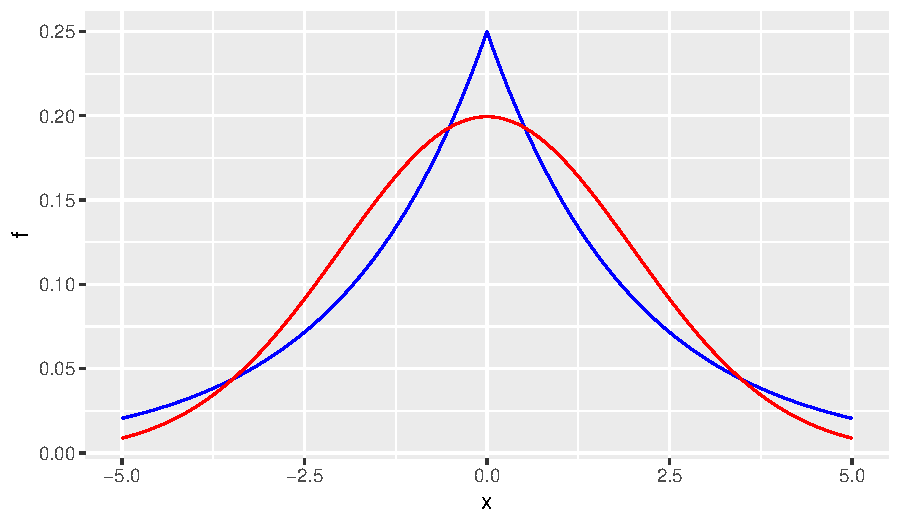
\includegraphics[width=\maxwidth]{figure/p2plot1-1} 
\end{knitrout}
\caption{Laplace distribution with superimposed Gaussian distribution}
\label{p2plot1}
\end{center}
\end{figure}
Compared to the Guassian distribution, the Laplace one has higher kurtosis. In other terms, with the same mean, it has a higher peak. Moreover, we can observe fatter tails within the Laplae distribution, compared to its Gaussian counterpart. \\
I might be wrong here, the variance of the Laplace distribution reminds me of the two exponential distributions that face two opposite directions. I assume that if the data is following this distribution, we'd see more values in the tails of the distribution and at its mean.

  \item Conduct a simulation study using the Laplace distribution. To do so, 
  complete the following 1000 times and report the proportion of times the
  data lead to a rejection of the null hypothesis.\\
  
  The most efficient way to complete this question (including the other parts)
  is to write a function that completes the following. 
  \begin{itemize}
    \item \textbf{Input:} 
    \begin{itemize}
      \item \texttt{rand.n=FALSE} -- a logical object denoting whether the sample
                                     size is random or not. False by default.
                                     See part (f).
      \item \texttt{rand.s=FALSE} -- a logical object denoting whether the dispersion
                                     equal or not not. False by default. See part (g).
      \item \texttt{equal.m=TRUE} -- a logical object denoting whether the location
                                     parameters should be equal (part b) or different 
                                     (part c). TRUE by default. 
      \item \texttt{n=5} -- the desired sample size if not random. Five by default.
    \end{itemize}
    \item \textbf{Loop the following tasks 1000 times:}
    \begin{itemize}
      \item Generate $t=4$ samples of size $n$ drawn independently from the 
        laplace distribution with $m$ and $s$ which can be done using 
        \texttt{rlaplace()} function from the rmutil package \citep{rmutil}. Specify
        $n$, $m$, and $s$ based on the values of the
        logical variables described above.
      \item Perform the ANOVA procedure on these generated data.
      \item Store whether the test resulted in a rejected null hypothesis or not.
    \end{itemize}
    \item \textbf{Return:}
    \begin{itemize}
      \item Your function should return the proportion of the 1000 ANOVA tests
      that resulted in a rejected null hypothesis.
    \end{itemize}
  \end{itemize}
    Comment on the results of this simulation completed in the default case where
  $m_1=m_2=m_3=m_4=0$, $s_1=s_2=s_3=s_4=2$, and $n_1=n_2=n_3=n_4=5$
  
\begin{knitrout}
\definecolor{shadecolor}{rgb}{0.969, 0.969, 0.969}\color{fgcolor}\begin{kframe}
\begin{alltt}
\hlkwd{library}\hlstd{(rstatix)}

\hlcom{#Body of the function}
\hlstd{aovFunc} \hlkwb{<-} \hlkwa{function}\hlstd{(}\hlkwc{rand.n}\hlstd{=}\hlnum{FALSE}\hlstd{,} \hlkwc{rand.s}\hlstd{=}\hlnum{FALSE}\hlstd{,} \hlkwc{equal.m}\hlstd{=}\hlnum{TRUE}\hlstd{,} \hlkwc{n}\hlstd{=}\hlnum{5}\hlstd{,} \hlkwc{loop}\hlstd{=}\hlnum{0}\hlstd{,}
                    \hlkwc{welch}\hlstd{=}\hlnum{FALSE}\hlstd{)\{}
  \hlstd{alpha}\hlkwb{<-}\hlnum{0.05}
  \hlstd{count}\hlkwb{=}\hlnum{0}
  \hlcom{#if random number of n is true, we'd use random number }
  \hlcom{#from uniform distribution}
  \hlkwa{if}\hlstd{(rand.n)\{}
    \hlstd{n1}\hlkwb{=}\hlkwd{round}\hlstd{(}\hlkwd{runif}\hlstd{(}\hlnum{1}\hlstd{,} \hlkwc{min}\hlstd{=}\hlnum{5}\hlstd{,} \hlkwc{max}\hlstd{=}\hlnum{100}\hlstd{),}\hlnum{0}\hlstd{)}
    \hlstd{n2}\hlkwb{=}\hlkwd{round}\hlstd{(}\hlkwd{runif}\hlstd{(}\hlnum{1}\hlstd{,} \hlkwc{min}\hlstd{=}\hlnum{5}\hlstd{,} \hlkwc{max}\hlstd{=}\hlnum{100}\hlstd{),}\hlnum{0}\hlstd{)}
    \hlstd{n3}\hlkwb{=}\hlkwd{round}\hlstd{(}\hlkwd{runif}\hlstd{(}\hlnum{1}\hlstd{,} \hlkwc{min}\hlstd{=}\hlnum{5}\hlstd{,} \hlkwc{max}\hlstd{=}\hlnum{100}\hlstd{),}\hlnum{0}\hlstd{)}
    \hlstd{n4}\hlkwb{=}\hlkwd{round}\hlstd{(}\hlkwd{runif}\hlstd{(}\hlnum{1}\hlstd{,} \hlkwc{min}\hlstd{=}\hlnum{5}\hlstd{,} \hlkwc{max}\hlstd{=}\hlnum{100}\hlstd{),}\hlnum{0}\hlstd{)}
  \hlstd{\}}
  \hlcom{#else: use the number passed on within the function (default: 5)}
  \hlkwa{else}\hlstd{\{}
    \hlstd{n1}\hlkwb{=}\hlstd{n}
    \hlstd{n2}\hlkwb{=}\hlstd{n}
    \hlstd{n3}\hlkwb{=}\hlstd{n}
    \hlstd{n4}\hlkwb{=}\hlstd{n}
  \hlstd{\}}

  \hlkwa{if}\hlstd{(rand.s)\{}
    \hlstd{s1}\hlkwb{=}\hlkwd{rgamma}\hlstd{(}\hlnum{1}\hlstd{,} \hlnum{2}\hlstd{,} \hlnum{1}\hlstd{)}
    \hlstd{s2}\hlkwb{=}\hlkwd{rgamma}\hlstd{(}\hlnum{1}\hlstd{,} \hlnum{2}\hlstd{,} \hlnum{1}\hlstd{)}
    \hlstd{s3}\hlkwb{=}\hlkwd{rgamma}\hlstd{(}\hlnum{1}\hlstd{,} \hlnum{2}\hlstd{,} \hlnum{1}\hlstd{)}
    \hlstd{s4}\hlkwb{=}\hlkwd{rgamma}\hlstd{(}\hlnum{1}\hlstd{,} \hlnum{2}\hlstd{,} \hlnum{1}\hlstd{)}
  \hlstd{\}}\hlkwa{else}\hlstd{\{}
    \hlstd{s1}\hlkwb{=}\hlnum{2}
    \hlstd{s2}\hlkwb{=}\hlnum{2}
    \hlstd{s3}\hlkwb{=}\hlnum{2}
    \hlstd{s4}\hlkwb{=}\hlnum{2}
  \hlstd{\}}
  \hlkwa{for}\hlstd{(i} \hlkwa{in} \hlnum{1}\hlopt{:}\hlstd{loop)\{}
    \hlkwa{if}\hlstd{(equal.m)\{}
      \hlcom{#if mean is equal, pass 0 to the function}
      \hlstd{t1}\hlkwb{<-}\hlkwd{rlaplace}\hlstd{(}\hlkwc{n}\hlstd{=n1,} \hlkwc{m}\hlstd{=}\hlnum{0}\hlstd{,} \hlkwc{s}\hlstd{=s1)}
      \hlstd{label1}\hlkwb{<-}\hlstr{"T1"}

      \hlstd{t2}\hlkwb{<-}\hlkwd{rlaplace}\hlstd{(}\hlkwc{n}\hlstd{=n2,} \hlkwc{m}\hlstd{=}\hlnum{0}\hlstd{,} \hlkwc{s}\hlstd{=s2)}
      \hlstd{label2}\hlkwb{<-}\hlstr{"T2"}

      \hlstd{t3}\hlkwb{<-}\hlkwd{rlaplace}\hlstd{(}\hlkwc{n}\hlstd{=n3,} \hlkwc{m}\hlstd{=}\hlnum{0}\hlstd{,} \hlkwc{s}\hlstd{=s3)}
      \hlstd{label3}\hlkwb{<-}\hlstr{"T3"}

      \hlstd{t4}\hlkwb{<-}\hlkwd{rlaplace}\hlstd{(}\hlkwc{n}\hlstd{=n4,} \hlkwc{m}\hlstd{=}\hlnum{0}\hlstd{,} \hlkwc{s}\hlstd{=s4)}
      \hlstd{label4}\hlkwb{<-}\hlstr{"T4"}
    \hlstd{\}}

    \hlkwa{else}\hlstd{\{}
      \hlcom{#else: pass 1 to the last function}
      \hlstd{t1}\hlkwb{<-}\hlkwd{rlaplace}\hlstd{(}\hlkwc{n}\hlstd{=n1,} \hlkwc{m}\hlstd{=}\hlnum{0}\hlstd{,} \hlkwc{s}\hlstd{=s1)}
      \hlstd{label1}\hlkwb{<-}\hlstr{"T1"}

      \hlstd{t2}\hlkwb{<-}\hlkwd{rlaplace}\hlstd{(}\hlkwc{n}\hlstd{=n2,} \hlkwc{m}\hlstd{=}\hlnum{0}\hlstd{,} \hlkwc{s}\hlstd{=s2)}
      \hlstd{label2}\hlkwb{<-}\hlstr{"T2"}

      \hlstd{t3}\hlkwb{<-}\hlkwd{rlaplace}\hlstd{(}\hlkwc{n}\hlstd{=n3,} \hlkwc{m}\hlstd{=}\hlnum{0}\hlstd{,} \hlkwc{s}\hlstd{=s3)}
      \hlstd{label3}\hlkwb{<-}\hlstr{"T3"}

      \hlstd{t4}\hlkwb{<-}\hlkwd{rlaplace}\hlstd{(}\hlkwc{n}\hlstd{=n4,} \hlkwc{m}\hlstd{=}\hlnum{1}\hlstd{,} \hlkwc{s}\hlstd{=s4)}
      \hlstd{label4}\hlkwb{<-}\hlstr{"T4"}
    \hlstd{\}}


    \hlcom{#passing the data with labels}
    \hlstd{dat}\hlkwb{<-}\hlkwd{data.frame}\hlstd{(}\hlkwc{value}\hlstd{=}\hlkwd{c}\hlstd{(t1, t2, t3, t4),}
                    \hlkwc{group}\hlstd{=}\hlkwd{c}\hlstd{(}\hlkwd{rep}\hlstd{(}\hlkwd{c}\hlstd{(}\hlstr{"T1"}\hlstd{,} \hlstr{"T2"}\hlstd{,} \hlstr{"T3"}\hlstd{,} \hlstr{"T4"}\hlstd{),}
                                                         \hlkwc{times}\hlstd{=}\hlkwd{c}\hlstd{(}\hlkwd{length}\hlstd{(t1),}
                                                                 \hlkwd{length}\hlstd{(t2),}
                                                                 \hlkwd{length}\hlstd{(t3),}
                                                                 \hlkwd{length}\hlstd{(t4)))))}
    \hlcom{#if we're not using Welch's ANOVA, go here}
    \hlkwa{if}\hlstd{(}\hlopt{!}\hlstd{welch)\{}
      \hlstd{anova}\hlkwb{<-}\hlkwd{summary}\hlstd{(}\hlkwd{aov}\hlstd{(value}\hlopt{~}\hlstd{group,} \hlkwc{data}\hlstd{=dat))}
      \hlstd{sum_test} \hlkwb{<-} \hlkwd{unlist}\hlstd{((anova))}
      \hlstd{p.value}\hlkwb{<-}\hlstd{sum_test[}\hlstr{"Pr(>F)1"}\hlstd{]}
      \hlcom{#print(p.value) #bugtest}
    \hlstd{\}}
    \hlcom{#Use Welch's ANOVA to assess its results when S is different}
    \hlcom{#NOT USED BUT STILL PRETTY COOL}
    \hlkwa{else}\hlstd{\{}
      \hlstd{anova_w}\hlkwb{<-}\hlkwd{welch_anova_test}\hlstd{(value}\hlopt{~}\hlstd{group,} \hlkwc{data}\hlstd{=dat)}
      \hlstd{p.value}\hlkwb{<-}\hlstd{anova_w}\hlopt{$}\hlstd{p}
    \hlstd{\}}

    \hlkwa{if}\hlstd{(p.value}\hlopt{<}\hlnum{0.05}\hlstd{)\{}
     \hlstd{count}\hlkwb{=}\hlstd{count}\hlopt{+}\hlnum{1}
    \hlstd{\}}
  \hlstd{\}}
  \hlstd{count}\hlopt{/}\hlstd{loop}
\hlstd{\}}
\end{alltt}
\end{kframe}
\end{knitrout}


\begin{knitrout}
\definecolor{shadecolor}{rgb}{0.969, 0.969, 0.969}\color{fgcolor}\begin{kframe}
\begin{alltt}
\hlkwd{aovFunc}\hlstd{(}\hlkwc{loop}\hlstd{=}\hlnum{1000}\hlstd{)}
\end{alltt}
\begin{verbatim}
## [1] 0.041
\end{verbatim}
\end{kframe}
\end{knitrout}
On average, it would appear there were only less than 2 percent of cases when the function had enough evidence to reject the null hypothesis. No wonder: the sample size was really small and the means were equal, so that's exactly what we'd expect to see.


  \item Repeat the simulation study in (b-d), except with different means; i.e.,
  $m_1=m_2=m_3=0$, and $m_4=1$. Comment on the results of this simulation.

\begin{knitrout}
\definecolor{shadecolor}{rgb}{0.969, 0.969, 0.969}\color{fgcolor}\begin{kframe}
\begin{alltt}
\hlkwd{aovFunc}\hlstd{(}\hlkwc{equal.m}\hlstd{=}\hlnum{FALSE}\hlstd{,} \hlkwc{loop}\hlstd{=}\hlnum{1000}\hlstd{)}
\end{alltt}
\begin{verbatim}
## [1] 0.075
\end{verbatim}
\end{kframe}
\end{knitrout}
Yet again, we're using a terribly small sample size, so, on average, only in less than 10 perecent of cases there was enough evidence to reject the null hypothesis. This suggests that ANOVA test majorly depends on its sample size. However, if we want to be certain in it, it would be highly advisable to simulate the same experiment with a bigger sample size.


\item Repeat the simulation study in (b-c), except with $n=15$. Comment on the results of this simulation.
\begin{knitrout}
\definecolor{shadecolor}{rgb}{0.969, 0.969, 0.969}\color{fgcolor}\begin{kframe}
\begin{alltt}
\hlkwd{aovFunc}\hlstd{(}\hlkwc{equal.m}\hlstd{=}\hlnum{TRUE}\hlstd{,} \hlkwc{loop}\hlstd{=}\hlnum{1000}\hlstd{,} \hlkwc{n}\hlstd{=}\hlnum{15}\hlstd{)}
\end{alltt}
\begin{verbatim}
## [1] 0.039
\end{verbatim}
\begin{alltt}
\hlkwd{aovFunc}\hlstd{(}\hlkwc{equal.m}\hlstd{=}\hlnum{FALSE}\hlstd{,} \hlkwc{loop}\hlstd{=}\hlnum{1000}\hlstd{,} \hlkwc{n}\hlstd{=}\hlnum{15}\hlstd{)}
\end{alltt}
\begin{verbatim}
## [1] 0.148
\end{verbatim}
\end{kframe}
\end{knitrout}
Now, when we increased the sample size to 15, we can see certain changes within our function. When the means are not equal, ANOVA is able to reject every second test. However, that is equal to a coin toss, so $n=15$ is still not enough to be certain in our results.

  \item Repeat the simulation study in (b-c), except with $n=50$.
  Comment on the results of this simulation.
\begin{knitrout}
\definecolor{shadecolor}{rgb}{0.969, 0.969, 0.969}\color{fgcolor}\begin{kframe}
\begin{alltt}
\hlkwd{aovFunc}\hlstd{(}\hlkwc{equal.m}\hlstd{=}\hlnum{TRUE}\hlstd{,} \hlkwc{loop}\hlstd{=}\hlnum{1000}\hlstd{,} \hlkwc{n}\hlstd{=}\hlnum{50}\hlstd{)}
\end{alltt}
\begin{verbatim}
## [1] 0.056
\end{verbatim}
\begin{alltt}
\hlkwd{aovFunc}\hlstd{(}\hlkwc{equal.m}\hlstd{=}\hlnum{FALSE}\hlstd{,} \hlkwc{loop}\hlstd{=}\hlnum{1000}\hlstd{,} \hlkwc{n}\hlstd{=}\hlnum{50}\hlstd{)}
\end{alltt}
\begin{verbatim}
## [1] 0.406
\end{verbatim}
\end{kframe}
\end{knitrout}
With a sample size as big as 50, on average, ANOVA is able to reject only less than 50-60 percent of hypothesis when the means are not equal. It implies that ANOVA is highly sensative to the sample size, and it's imperative for researchers to maintain it high! 

\item Repeat (b-e), except randomly select the sample size for each 
group by selecting $n$ from the uniform(5,100) distribution. This 
will help us assess the robustness of the equal sample size assumption
in the Laplace population distribution case. Comment on the results of 
this simulation.
\begin{knitrout}
\definecolor{shadecolor}{rgb}{0.969, 0.969, 0.969}\color{fgcolor}\begin{kframe}
\begin{alltt}
\hlkwd{aovFunc}\hlstd{(}\hlkwc{equal.m}\hlstd{=}\hlnum{TRUE}\hlstd{,} \hlkwc{rand.n}\hlstd{=}\hlnum{TRUE}\hlstd{,} \hlkwc{loop}\hlstd{=}\hlnum{1000}\hlstd{)}
\end{alltt}
\begin{verbatim}
## [1] 0.041
\end{verbatim}
\begin{alltt}
\hlkwd{aovFunc}\hlstd{(}\hlkwc{equal.m}\hlstd{=}\hlnum{FALSE}\hlstd{,} \hlkwc{rand.n}\hlstd{=}\hlnum{TRUE}\hlstd{,} \hlkwc{loop}\hlstd{=}\hlnum{1000}\hlstd{)}
\end{alltt}
\begin{verbatim}
## [1] 0.622
\end{verbatim}
\end{kframe}
\end{knitrout}
Throughout various runs of this function, I failed to notice consistently high results from ANOVA. It is true that, on average, ANOVA managed to reject 40-50\%+ of null hypothesis when means were not equal. However, it also failed to show consistently high results. I observed 20-30\% of rejected hypothesis as many times as I saw 50-70\% of rejected hypothesis. However, in the case of unequal sample size, I noticed that ANOVA did not show consistently worse results.

\item Repeat (b-f), except randomly select the dispersion for each 
  group by selecting $s$ from the gamma(2,1) distribution. This 
  will help us assess the robustness of the equal variance assumption
  in the Laplace population distribution case. Comment on the results of 
  this simulation.
\begin{knitrout}
\definecolor{shadecolor}{rgb}{0.969, 0.969, 0.969}\color{fgcolor}\begin{kframe}
\begin{alltt}
\hlkwd{aovFunc}\hlstd{(}\hlkwc{equal.m}\hlstd{=}\hlnum{TRUE}\hlstd{,} \hlkwc{rand.n}\hlstd{=}\hlnum{TRUE}\hlstd{,} \hlkwc{rand.s}\hlstd{=}\hlnum{TRUE}\hlstd{,} \hlkwc{loop}\hlstd{=}\hlnum{1000}\hlstd{)}
\end{alltt}
\begin{verbatim}
## [1] 0.132
\end{verbatim}
\begin{alltt}
\hlkwd{aovFunc}\hlstd{(}\hlkwc{equal.m}\hlstd{=}\hlnum{FALSE}\hlstd{,} \hlkwc{rand.n}\hlstd{=}\hlnum{TRUE}\hlstd{,} \hlkwc{rand.s}\hlstd{=}\hlnum{TRUE}\hlstd{,} \hlkwc{loop}\hlstd{=}\hlnum{1000}\hlstd{)}
\end{alltt}
\begin{verbatim}
## [1] 0.121
\end{verbatim}
\end{kframe}
\end{knitrout}
When dispersion is not equal (in addition to unequal sample size), ANOVA test manages to reject, on average, more less 50\% of the hypothesis when the means are not equal. So while in the previous case this result might have been higher than 50\%, an additional difference in variance greatly undermined the power of ANOVA test.

\item Write a loop that conducts this simulation when (1) $s$ is fixed and (2) 
when $s$ is random, for the case where the means are unequal. The loop should be 
with respect to $n$, and should run for $n=5$ to $n=200$.\\
\textbf{Note:} This can take some computation time, you'll want to run it and save 
the image as a .pdf so you can load it instead of rerunning the code.
\begin{knitrout}
\definecolor{shadecolor}{rgb}{0.969, 0.969, 0.969}\color{fgcolor}\begin{kframe}
\begin{alltt}
\hlstd{results}\hlkwb{<-}\hlkwd{c}\hlstd{()}
\hlstd{n}\hlkwb{<-}\hlnum{10}\hlopt{:}\hlnum{200}
\hlstd{y1}\hlkwb{<-}\hlkwd{c}\hlstd{()}
\hlstd{y2}\hlkwb{<-}\hlkwd{c}\hlstd{()}

\hlkwa{for}\hlstd{(i} \hlkwa{in} \hlnum{10}\hlopt{:}\hlnum{200}\hlstd{)\{}
  \hlkwd{print}\hlstd{(i)}
  \hlstd{unequal}\hlkwb{<-}\hlkwd{aovFunc}\hlstd{(}\hlkwc{equal.m}\hlstd{=}\hlnum{FALSE}\hlstd{,} \hlkwc{rand.s}\hlstd{=}\hlnum{TRUE}\hlstd{,} \hlkwc{loop}\hlstd{=}\hlnum{1000}\hlstd{,} \hlkwc{n}\hlstd{=i)}
  \hlstd{y1}\hlkwb{<-}\hlkwd{c}\hlstd{(y1, unequal)}
  \hlstd{equal}\hlkwb{<-}\hlkwd{aovFunc}\hlstd{(}\hlkwc{equal.m}\hlstd{=}\hlnum{FALSE}\hlstd{,} \hlkwc{rand.s}\hlstd{=}\hlnum{FALSE}\hlstd{,} \hlkwc{loop}\hlstd{=}\hlnum{1000}\hlstd{,} \hlkwc{n}\hlstd{=i)}
  \hlstd{y2}\hlkwb{<-}\hlkwd{c}\hlstd{(y2, equal)}
\hlstd{\}}
\hlstd{ggdat}\hlkwb{<-}\hlkwd{data.frame}\hlstd{(}\hlkwc{x}\hlstd{=n,} \hlkwc{equal.s}\hlstd{=y2,} \hlkwc{unequal.s}\hlstd{=y1)}
\end{alltt}
\end{kframe}
\end{knitrout}

\begin{figure}[H]
\begin{center}
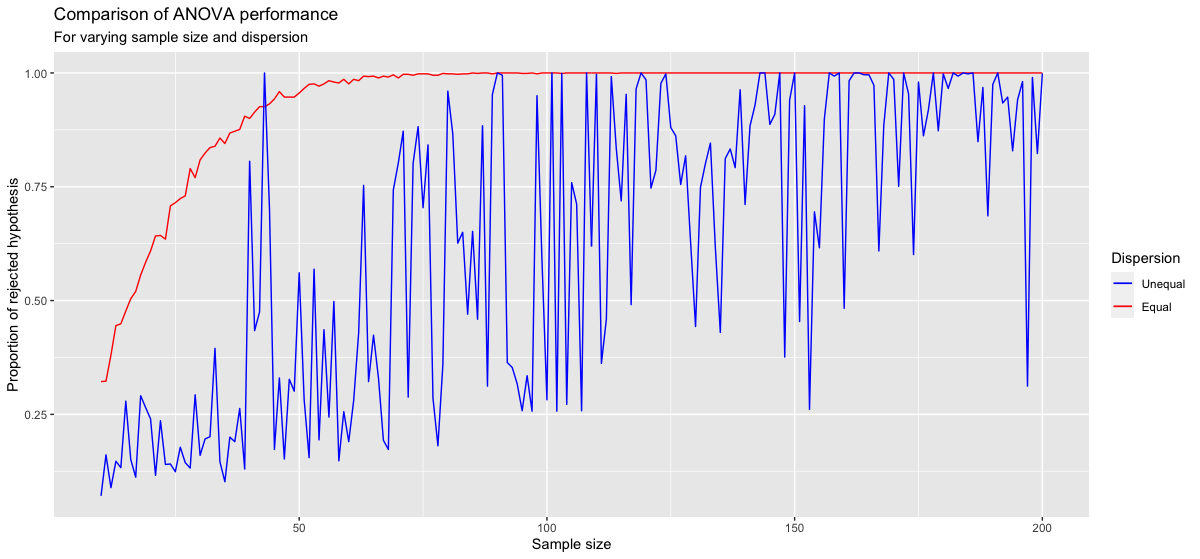
\includegraphics[scale=0.40]{Rplot.png}
\caption{The assessment of ANOVA performance on Laplace distribution}
\label{p2plot2}
\end{center}
\end{figure}

This graph provides enough evidence to make a conclusion that the variance assumption is far more important for ANOVA than the sample size assumption. We can observe that even with massive sample size the function with unequal variance keeps underpeforming, compared to the with the equal variance. Hence, the reason of using Welch's ANOVA — it will eliminate the assumption about the equal variance.

\end{enumerate}
\newpage
%%%%%%%%%%%%%%%%%%%%%%%%%%%%%%%%%%%%%%%%%%%%%%%%%%%%%%%%%%%%%%%%%%%%%%%%%%%%%%%
%%%%%%%%%%%%%%%%%%%%%%%%%%%%%%%%%%%%%%%%%%%%%%%%%%%%%%%%%%%%%%%%%%%%%%%%%%%%%%%
%%%%%%%%%  Question 3
%%%%%%%%%%%%%%%%%%%%%%%%%%%%%%%%%%%%%%%%%%%%%%%%%%%%%%%%%%%%%%%%%%%%%%%%%%%%%%%
%%%%%%%%%%%%%%%%%%%%%%%%%%%%%%%%%%%%%%%%%%%%%%%%%%%%%%%%%%%%%%%%%%%%%%%%%%%%%%%
  \item Complete the following parts. This will lead you through the simulation
  of data, fitting regression lines and evaluating the assumptions.
  \begin{enumerate}
  \item Fit a model to the following simulated data. Make observations about
  the model equation and the Pearson correlation.
\begin{knitrout}
\definecolor{shadecolor}{rgb}{0.969, 0.969, 0.969}\color{fgcolor}\begin{kframe}
\begin{alltt}
\hlstd{n}\hlkwb{=}\hlnum{500}
\hlstd{x}\hlkwb{<-}\hlkwd{sample}\hlstd{(}\hlkwc{x} \hlstd{=} \hlkwd{seq}\hlstd{(}\hlnum{0}\hlstd{,}\hlnum{5}\hlstd{,}\hlnum{0.01}\hlstd{),} \hlkwc{size}\hlstd{=n,} \hlkwc{replace}\hlstd{=T)}
\hlstd{y}\hlkwb{<-}\hlnum{5}\hlopt{*}\hlstd{x} \hlopt{+} \hlnum{3}
\end{alltt}
\end{kframe}
\end{knitrout}

\begin{figure}[H]
\begin{center}
\begin{knitrout}
\definecolor{shadecolor}{rgb}{0.969, 0.969, 0.969}\color{fgcolor}\begin{kframe}
\begin{alltt}
\hlstd{ggdat}\hlkwb{<-}\hlkwd{data.frame}\hlstd{(}\hlkwc{x}\hlstd{=x,} \hlkwc{y}\hlstd{=y)}
\hlkwd{ggplot}\hlstd{(ggdat,} \hlkwd{aes}\hlstd{(}\hlkwc{x}\hlstd{=x,} \hlkwc{y}\hlstd{=y))}\hlopt{+}
  \hlkwd{geom_smooth}\hlstd{(}\hlkwc{color}\hlstd{=}\hlstr{"blue"}\hlstd{,}
              \hlkwc{method}\hlstd{=}\hlstr{"lm"}\hlstd{,}
              \hlkwc{formula}\hlstd{=y}\hlopt{~}\hlstd{x)}\hlopt{+}
  \hlkwd{geom_point}\hlstd{(}\hlkwc{shape}\hlstd{=}\hlnum{1}\hlstd{,}
             \hlkwc{alpha}\hlstd{=}\hlnum{.3}\hlstd{)}\hlopt{+}
  \hlkwd{theme_bw}\hlstd{()}\hlopt{+}
  \hlkwd{annotate}\hlstd{(}\hlstr{"text"}\hlstd{,} \hlkwc{x}\hlstd{=}\hlnum{1}\hlstd{,} \hlkwc{y}\hlstd{=}\hlnum{22}\hlstd{,}
           \hlkwc{label}\hlstd{=}\hlkwd{paste}\hlstd{(}\hlstr{"Pearson correlation:"}\hlstd{,}
                       \hlkwd{cor}\hlstd{(x,y,}\hlkwc{method}\hlstd{=}\hlstr{"pearson"}\hlstd{),}\hlstr{"\textbackslash{}nPerfect!"}\hlstd{))}
\end{alltt}
\end{kframe}
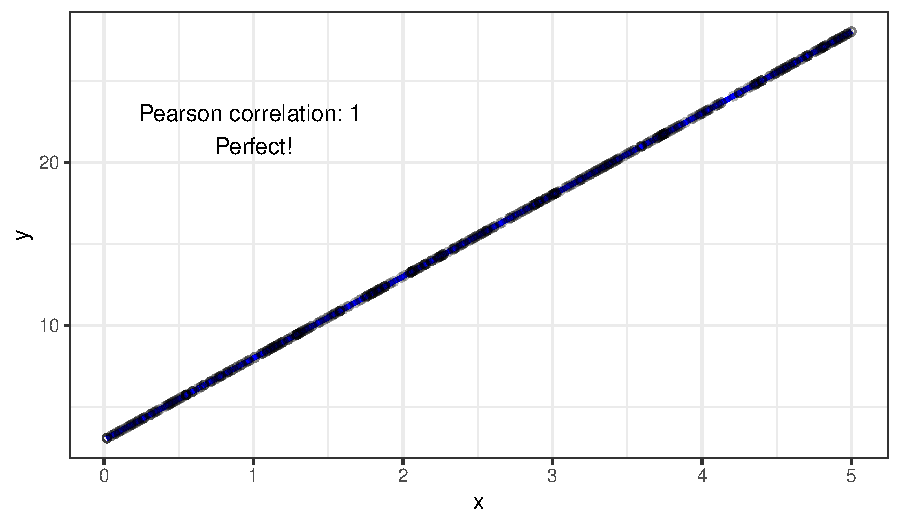
\includegraphics[width=\maxwidth]{figure/p3plot1-1} 
\end{knitrout}
\caption{Fitted model for \texttt{x} and \texttt{y}}
\label{p3plot1}
\end{center}
\end{figure}
We have the Pearson correlation of one! It means that our linear regression perfectly aligns with the data that we have!


  \item Fit a model to the following simulated data, now with added Normal error. Make
  observations about the model equation and the Pearson correlation in relation to (a).
\begin{knitrout}
\definecolor{shadecolor}{rgb}{0.969, 0.969, 0.969}\color{fgcolor}\begin{kframe}
\begin{alltt}
\hlstd{e}\hlkwb{<-}\hlkwd{rnorm}\hlstd{(}\hlkwc{n}\hlstd{=n,}\hlkwc{mean}\hlstd{=}\hlnum{0}\hlstd{,}\hlkwc{sd}\hlstd{=}\hlnum{3}\hlstd{)}
\hlstd{y2}\hlkwb{<-}\hlnum{5}\hlopt{*}\hlstd{x} \hlopt{+} \hlnum{3} \hlopt{+} \hlstd{e}
\end{alltt}
\end{kframe}
\end{knitrout}

\begin{figure}[H]
\begin{center}
\begin{knitrout}
\definecolor{shadecolor}{rgb}{0.969, 0.969, 0.969}\color{fgcolor}\begin{kframe}
\begin{alltt}
\hlstd{ggdat}\hlkwb{<-}\hlkwd{data.frame}\hlstd{(}\hlkwc{x}\hlstd{=x,} \hlkwc{y}\hlstd{=y2)}
\hlkwd{ggplot}\hlstd{(ggdat,} \hlkwd{aes}\hlstd{(}\hlkwc{x}\hlstd{=x,} \hlkwc{y}\hlstd{=y))}\hlopt{+}
  \hlkwd{geom_smooth}\hlstd{(}\hlkwc{color}\hlstd{=}\hlstr{"blue"}\hlstd{,}
              \hlkwc{method}\hlstd{=}\hlstr{"lm"}\hlstd{,}
              \hlkwc{formula}\hlstd{=y}\hlopt{~}\hlstd{x)}\hlopt{+}
  \hlkwd{geom_point}\hlstd{(}\hlkwc{shape}\hlstd{=}\hlnum{1}\hlstd{,}
             \hlkwc{alpha}\hlstd{=}\hlnum{.3}\hlstd{)}\hlopt{+}
  \hlkwd{theme_bw}\hlstd{()}\hlopt{+}
  \hlkwd{annotate}\hlstd{(}\hlstr{"text"}\hlstd{,} \hlkwc{x}\hlstd{=}\hlnum{1}\hlstd{,} \hlkwc{y}\hlstd{=}\hlnum{25}\hlstd{,}
           \hlkwc{label}\hlstd{=}\hlkwd{paste}\hlstd{(}\hlstr{"Pearson correlation:"}\hlstd{,}
                       \hlkwd{round}\hlstd{(}\hlkwd{cor}\hlstd{(x,y2,}\hlkwc{method}\hlstd{=}\hlstr{"pearson"}\hlstd{),}\hlnum{2}\hlstd{),}\hlstr{"\textbackslash{}nHighly correlated!"}\hlstd{))}\hlopt{+}
  \hlkwd{labs}\hlstd{(}\hlkwc{title}\hlstd{=}\hlstr{"Fitting the linear regression model"}\hlstd{,}
       \hlkwc{subtitle}\hlstd{=}\hlstr{"With simulated data with added Normal error"}\hlstd{)}
\end{alltt}
\end{kframe}
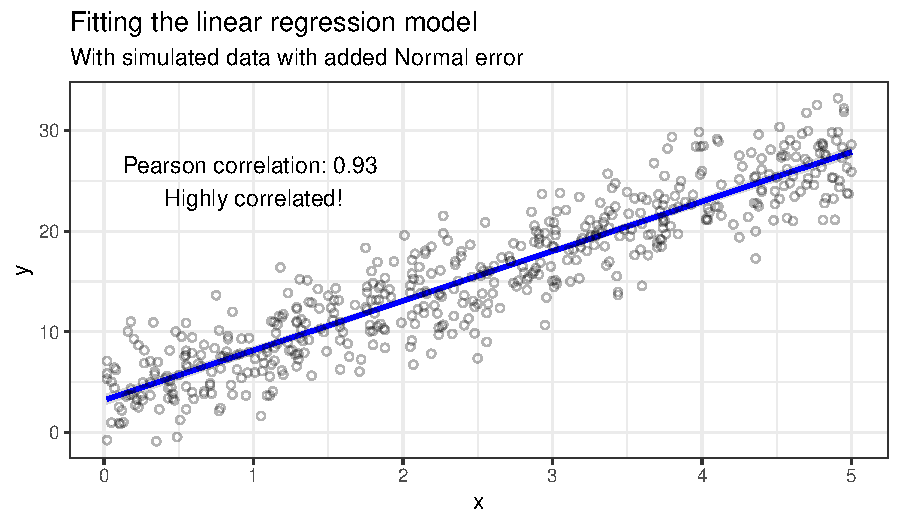
\includegraphics[width=\maxwidth]{figure/p3plot2-1} 
\end{knitrout}
\caption{Fitted model for \texttt{x} and \texttt{y2}}
\label{p3plot2}
\end{center}
\end{figure}

Based on the visual inspection, the data in the figure \ref{p3plot2} is homoscedastic (equal variance), and the Pearson correlation is 0.93! However, in order to be completely sure in our assessment, we ought to dig deeper and build additional graphs!

  \item In the model of part (b), evaluate the normality and homogeneity of error terms. Note 
  that we know both of these items to be true since we've taken $\epsilon \sim 
  \textrm{N}(\mu=0,\sigma=3)$.
\begin{knitrout}
\definecolor{shadecolor}{rgb}{0.969, 0.969, 0.969}\color{fgcolor}\begin{kframe}
\begin{alltt}
\hlcom{#Preparing the functions!}
\hlkwd{library}\hlstd{(patchwork)}
\hlkwd{source}\hlstd{(}\hlstr{"https://cipolli.com/students/code/plotResiduals.R"}\hlstd{)}
\hlkwd{source}\hlstd{(}\hlstr{"https://cipolli.com/students/code/plotInfluence.R"}\hlstd{)}
\end{alltt}
\end{kframe}
\end{knitrout}

We'll start off with building \texttt{lm()} model for our data!

\begin{knitrout}
\definecolor{shadecolor}{rgb}{0.969, 0.969, 0.969}\color{fgcolor}\begin{kframe}
\begin{alltt}
\hlstd{model1} \hlkwb{<-} \hlkwd{lm}\hlstd{(y2}\hlopt{~}\hlstd{x)}
\end{alltt}
\end{kframe}
\end{knitrout}

\begin{figure}[H]
\begin{center}
\begin{knitrout}
\definecolor{shadecolor}{rgb}{0.969, 0.969, 0.969}\color{fgcolor}\begin{kframe}
\begin{alltt}
\hlkwd{plotResiduals}\hlstd{(model1)}
\end{alltt}
\end{kframe}
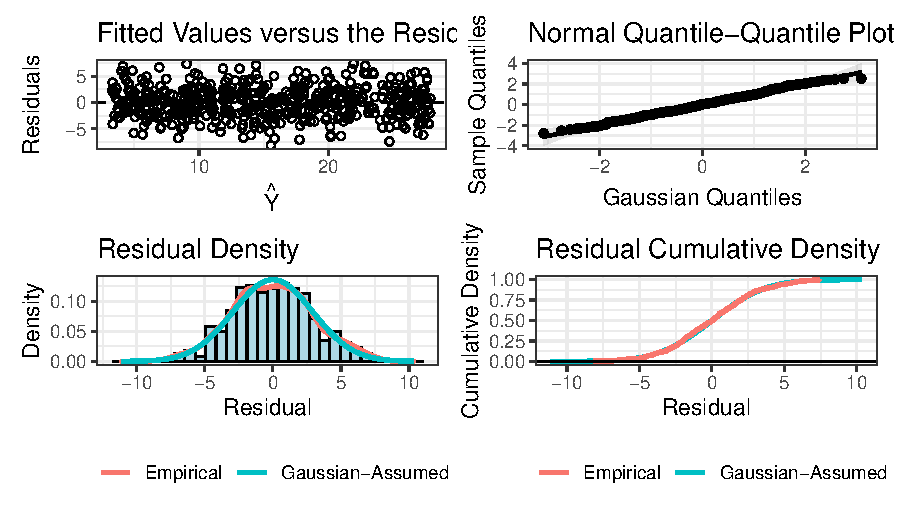
\includegraphics[width=\maxwidth]{figure/p3plot3-1} 
\end{knitrout}
\caption{Simulated data: \textbf{Top Left:} A fitted versus residual scatterplot.
\textbf{Top Right:} A normal q-q plot of the residuals. \textbf{Bottom Left:} A histogram of the residuals with a density curve. \textbf{Bottom Right:} A cumulitive density plot with an empirical density plot.}
\label{p3plot3}
\end{center}
\end{figure}

Looking at plot \ref{p3plot3}, it's obvious that residuals are Gaussian: q-q plot looks normal and assumed Gaussian distribution follows closely the observed distribution. In the fitted values versus residuals plot, we can observe that the data has equal variance. 

\item Fit a model to the following simulated data, now with added exponential error.
  Make observations about the model equation and the Pearson correlation in relation 
  to the model of part (b).
\begin{knitrout}
\definecolor{shadecolor}{rgb}{0.969, 0.969, 0.969}\color{fgcolor}\begin{kframe}
\begin{alltt}
\hlstd{e}\hlkwb{<-}\hlkwd{rexp}\hlstd{(}\hlkwc{n}\hlstd{=n,}\hlkwc{rate} \hlstd{=} \hlnum{1}\hlopt{/}\hlnum{2}\hlstd{)}
\hlstd{y3}\hlkwb{<-}\hlnum{5}\hlopt{*}\hlstd{x} \hlopt{+} \hlnum{3} \hlopt{+} \hlstd{e}
\end{alltt}
\end{kframe}
\end{knitrout}

\begin{figure}[H]
\begin{center}
\begin{knitrout}
\definecolor{shadecolor}{rgb}{0.969, 0.969, 0.969}\color{fgcolor}\begin{kframe}
\begin{alltt}
\hlstd{ggdat}\hlkwb{<-}\hlkwd{data.frame}\hlstd{(}\hlkwc{x}\hlstd{=x,} \hlkwc{y}\hlstd{=y3)}
\hlkwd{ggplot}\hlstd{(ggdat,} \hlkwd{aes}\hlstd{(}\hlkwc{x}\hlstd{=x,} \hlkwc{y}\hlstd{=y3))}\hlopt{+}
  \hlkwd{geom_smooth}\hlstd{(}\hlkwc{color}\hlstd{=}\hlstr{"blue"}\hlstd{,}
              \hlkwc{method}\hlstd{=}\hlstr{"lm"}\hlstd{,}
              \hlkwc{formula}\hlstd{=y}\hlopt{~}\hlstd{x)}\hlopt{+}
  \hlkwd{geom_point}\hlstd{(}\hlkwc{shape}\hlstd{=}\hlnum{1}\hlstd{,}
             \hlkwc{alpha}\hlstd{=}\hlnum{.3}\hlstd{)}\hlopt{+}
  \hlkwd{theme_bw}\hlstd{()}\hlopt{+}
  \hlkwd{annotate}\hlstd{(}\hlstr{"text"}\hlstd{,} \hlkwc{x}\hlstd{=}\hlnum{1}\hlstd{,} \hlkwc{y}\hlstd{=}\hlnum{25}\hlstd{,}
           \hlkwc{label}\hlstd{=}\hlkwd{paste}\hlstd{(}\hlstr{"Pearson correlation:"}\hlstd{,}
                       \hlkwd{round}\hlstd{(}\hlkwd{cor}\hlstd{(x,y3,}\hlkwc{method}\hlstd{=}\hlstr{"pearson"}\hlstd{),}\hlnum{2}\hlstd{),}\hlstr{"\textbackslash{}nHighly correlated!"}\hlstd{))}\hlopt{+}
  \hlkwd{labs}\hlstd{(}\hlkwc{title}\hlstd{=}\hlstr{"Fitting the linear regression model"}\hlstd{,}
       \hlkwc{subtitle}\hlstd{=}\hlstr{"With simulated data with added exponential error"}\hlstd{)}
\end{alltt}
\end{kframe}
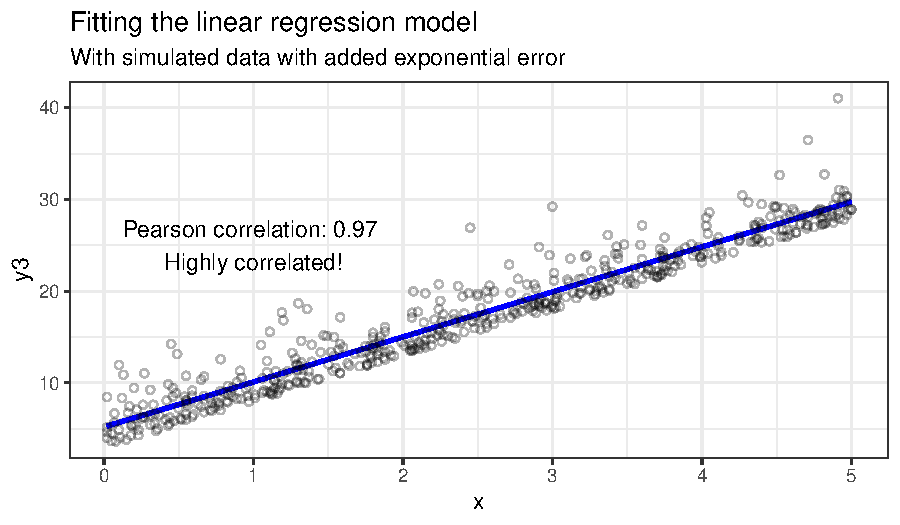
\includegraphics[width=\maxwidth]{figure/p3plot4-1} 
\end{knitrout}
\caption{Fitted model for \texttt{x} and \texttt{y3}}
\label{p3plot4}
\end{center}
\end{figure}
The Pearson correlation tells us that values \texttt{x} and \texttt{y3} are highly correlated. Through visual inspection, it's easier to notice that the data apepars skewed towards one side. I would assume that the constant variance assumption holds true though! However, yet again, we ought to build more plots to assess the validity of my assumptions.

  \item In the model of part (d), evaluate the normality and homogeneity of error 
  terms. Note that we know that common variance is true but we've taken $\epsilon \sim 
  \textrm{exp}(\beta=2)$.
\begin{knitrout}
\definecolor{shadecolor}{rgb}{0.969, 0.969, 0.969}\color{fgcolor}\begin{kframe}
\begin{alltt}
\hlstd{model2} \hlkwb{<-} \hlkwd{lm}\hlstd{(y3}\hlopt{~}\hlstd{x)}
\hlcom{#It's a skewed normal distribution, but it's homoscedastic!}
\end{alltt}
\end{kframe}
\end{knitrout}

\begin{figure}[H]
\begin{center}
\begin{knitrout}
\definecolor{shadecolor}{rgb}{0.969, 0.969, 0.969}\color{fgcolor}\begin{kframe}
\begin{alltt}
\hlkwd{plotResiduals}\hlstd{(model2)}
\end{alltt}
\end{kframe}
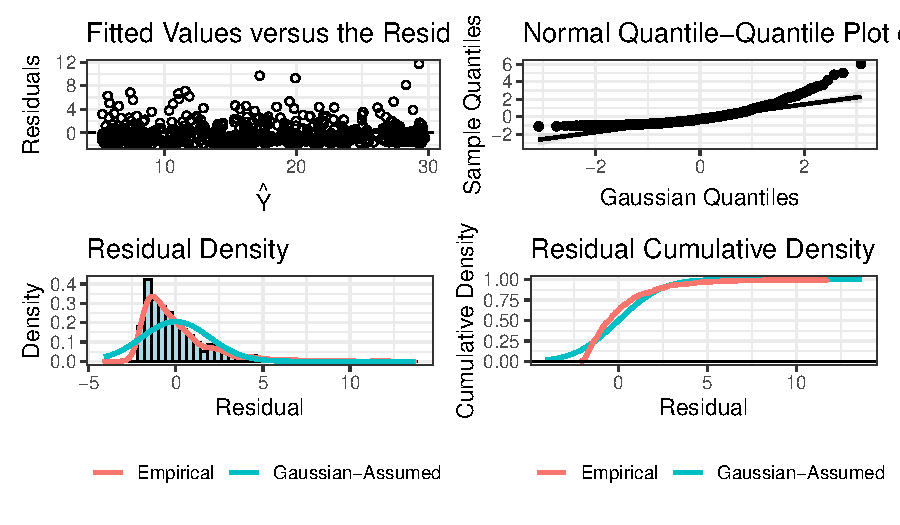
\includegraphics[width=\maxwidth]{figure/p3plot5-1} 
\end{knitrout}
\caption{Simulated data: \textbf{Top Left:} A fitted versus residual scatterplot.
\textbf{Top Right:} A normal q-q plot of the residuals. \textbf{Bottom Left:} A histogram of the residuals with a density curve. \textbf{Bottom Right:} A cumulitive density plot with an empirical density plot.}
\label{p3plot5}
\end{center}
\end{figure}

The first thing that's worth noting is that my visual inspection was correct. The Residual density histogram shows the skewed data. Moreoever, the ends of the q-q plot support this observation. However, it's worth noting that data appears to be homoscedastic! These differences lead to the observed differences in the cumulative density. We can be confident that errors do not follow the normal distribution!

\item Fit a model to the following simulated data, now with added Heteroskedastic
normal error. Make observations about the model equation and the Pearson correlation
in relation to the model of part (b).
\begin{knitrout}
\definecolor{shadecolor}{rgb}{0.969, 0.969, 0.969}\color{fgcolor}\begin{kframe}
\begin{alltt}
\hlstd{x4}\hlkwb{<-}\hlstd{x[}\hlkwd{order}\hlstd{(x)]}
\hlstd{e}\hlkwb{<-}\hlkwd{rnorm}\hlstd{(}\hlkwc{n}\hlstd{=n,}\hlkwc{mean}\hlstd{=}\hlnum{0}\hlstd{,}\hlkwc{sd}\hlstd{=}\hlkwd{c}\hlstd{(}\hlkwd{rep}\hlstd{(}\hlnum{1}\hlstd{,n}\hlopt{/}\hlnum{2}\hlstd{),}\hlkwd{rep}\hlstd{(}\hlnum{3}\hlstd{,n}\hlopt{/}\hlnum{2}\hlstd{)))}
\hlstd{y4}\hlkwb{<-}\hlnum{5}\hlopt{*}\hlstd{x4} \hlopt{+} \hlnum{3} \hlopt{+} \hlstd{e}
\end{alltt}
\end{kframe}
\end{knitrout}

\begin{figure}[H]
\begin{center}
\begin{knitrout}
\definecolor{shadecolor}{rgb}{0.969, 0.969, 0.969}\color{fgcolor}\begin{kframe}
\begin{alltt}
\hlstd{ggdat}\hlkwb{<-}\hlkwd{data.frame}\hlstd{(}\hlkwc{x}\hlstd{=x4,} \hlkwc{y}\hlstd{=y4)}
\hlkwd{ggplot}\hlstd{(ggdat,} \hlkwd{aes}\hlstd{(}\hlkwc{x}\hlstd{=x,} \hlkwc{y}\hlstd{=y))}\hlopt{+}
  \hlkwd{geom_smooth}\hlstd{(}\hlkwc{color}\hlstd{=}\hlstr{"blue"}\hlstd{,}
              \hlkwc{method}\hlstd{=}\hlstr{"lm"}\hlstd{,}
              \hlkwc{formula}\hlstd{=y}\hlopt{~}\hlstd{x)}\hlopt{+}
  \hlkwd{geom_point}\hlstd{(}\hlkwc{shape}\hlstd{=}\hlnum{1}\hlstd{,}
             \hlkwc{alpha}\hlstd{=}\hlnum{.3}\hlstd{)}\hlopt{+}
  \hlkwd{theme_bw}\hlstd{()}\hlopt{+}
  \hlkwd{annotate}\hlstd{(}\hlstr{"text"}\hlstd{,} \hlkwc{x}\hlstd{=}\hlnum{1}\hlstd{,} \hlkwc{y}\hlstd{=}\hlnum{25}\hlstd{,}
           \hlkwc{label}\hlstd{=}\hlkwd{paste}\hlstd{(}\hlstr{"Pearson correlation:"}\hlstd{,}
                       \hlkwd{round}\hlstd{(}\hlkwd{cor}\hlstd{(x4,y4,}\hlkwc{method}\hlstd{=}\hlstr{"pearson"}\hlstd{),}\hlnum{2}\hlstd{),}\hlstr{"\textbackslash{}nHighly correlated!"}\hlstd{))}\hlopt{+}
  \hlkwd{labs}\hlstd{(}\hlkwc{title}\hlstd{=}\hlstr{"Fitting the linear regression model"}\hlstd{,}
       \hlkwc{subtitle}\hlstd{=}\hlstr{"With simulated data with added heteroskedastic normal error"}\hlstd{)}
\end{alltt}
\end{kframe}
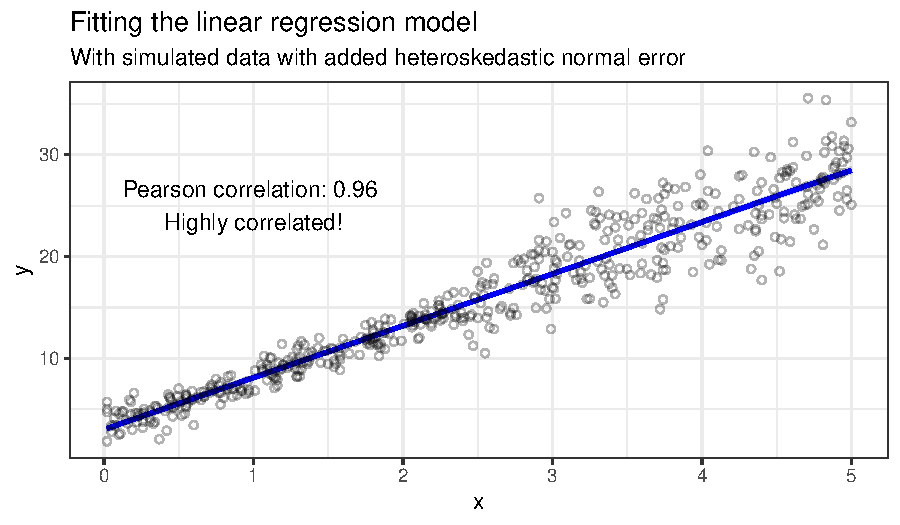
\includegraphics[width=\maxwidth]{figure/p3plot6-1} 
\end{knitrout}
\caption{Fitted model for \texttt{x} and \texttt{y4}}
\label{p3plot6}
\end{center}
\end{figure}

The Pearson correlation keeps showing that values of \texttt{x} and \texttt{y} are highly correlated. However, it's important to stress that even the brief visual inspection allows us to notice the heteroskedastic nature of the data that we are working with! It would appear than variance is different for the values that are lower than 2.5 and the ones that are higher than that. 

  \item In the model of part (f), evaluate the normality and homogeneity of error terms. Note
  that we know that normality of error terms is true, but $\epsilon \sim 
  \textrm{N}(\mu=0,\sigma=1)$ for $x<\widehat{m}$ and $\epsilon \sim 
  \textrm{N}(\mu=0,\sigma=3)$ for $x>\widehat{m}$.
\begin{knitrout}
\definecolor{shadecolor}{rgb}{0.969, 0.969, 0.969}\color{fgcolor}\begin{kframe}
\begin{alltt}
\hlstd{model3} \hlkwb{<-} \hlkwd{lm}\hlstd{(y4}\hlopt{~}\hlstd{x4)}
\end{alltt}
\end{kframe}
\end{knitrout}


\begin{figure}[H]
\begin{center}
\begin{knitrout}
\definecolor{shadecolor}{rgb}{0.969, 0.969, 0.969}\color{fgcolor}\begin{kframe}
\begin{alltt}
\hlkwd{plotResiduals}\hlstd{(model3)}
\end{alltt}
\end{kframe}
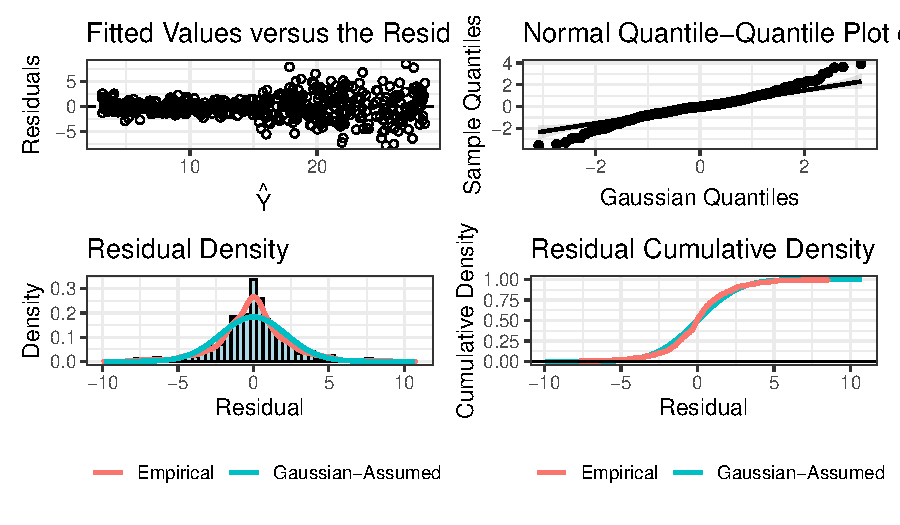
\includegraphics[width=\maxwidth]{figure/p3plot7-1} 
\end{knitrout}
\caption{Simulated data: \textbf{Top Left:} A fitted versus residual scatterplot.
\textbf{Top Right:} A normal q-q plot of the residuals. \textbf{Bottom Left:} A histogram of the residuals with a density curve. \textbf{Bottom Right:} A cumulitive density plot with an empirical density plot.}
\label{p3plot7}
\end{center}
\end{figure}
\end{enumerate}

Unlike the plot\ref{p3plot5} that we've been working on before, the plot\ref{p3plot7}'s errors follow actually follow the normal distribution. The assumed Gaussian distribution fits incredibly well to the observed empirical distribution. However, this time we ought to pay attention to the the fitted values versus residuals plot. It shows the change in variance, implying that the data is heteroskedastic!

%%%%%%%%%%%%%%%%%%%%%%%%%%%%%%%%%%%%%%%%%%%%%%%%%%%%%%%%%%%%%%%%%%%%%%%%%%%%%%%
%%%%%%%%%%%%%%%%%%%%%%%%%%%%%%%%%%%%%%%%%%%%%%%%%%%%%%%%%%%%%%%%%%%%%%%%%%%%%%%
%%%%%%%%%  Question 4
%%%%%%%%%%%%%%%%%%%%%%%%%%%%%%%%%%%%%%%%%%%%%%%%%%%%%%%%%%%%%%%%%%%%%%%%%%%%%%%
%%%%%%%%%%%%%%%%%%%%%%%%%%%%%%%%%%%%%%%%%%%%%%%%%%%%%%%%%%%%%%%%%%%%%%%%%%%%%%%
\item Consider the following simulation.
  \begin{enumerate}
    \item Plot the data simulated below. Assess the linear relationship.
\begin{knitrout}
\definecolor{shadecolor}{rgb}{0.969, 0.969, 0.969}\color{fgcolor}\begin{kframe}
\begin{alltt}
\hlkwd{library}\hlstd{(tidyverse)}
\hlkwd{set.seed}\hlstd{(}\hlnum{7272}\hlstd{)}
\hlstd{n}\hlkwb{<-}\hlnum{50}
\hlstd{ggdat} \hlkwb{<-} \hlkwd{data.frame}\hlstd{(}\hlkwc{x}\hlstd{=}\hlkwd{sample}\hlstd{(}\hlkwc{x}\hlstd{=}\hlkwd{seq}\hlstd{(}\hlnum{0}\hlstd{,}\hlnum{100}\hlstd{,}\hlnum{0.01}\hlstd{),}\hlkwc{size}\hlstd{=n,}\hlkwc{replace}\hlstd{=}\hlnum{TRUE}\hlstd{))} \hlopt
  \hlkwd{mutate}\hlstd{(}\hlkwc{y}\hlstd{=}\hlnum{3.5}\hlopt{+}\hlnum{2.1}\hlopt{*}\hlstd{x}\hlopt{+}\hlkwd{rnorm}\hlstd{(}\hlkwc{n}\hlstd{=n,}\hlkwc{mean}\hlstd{=}\hlnum{0}\hlstd{,}\hlkwc{sd}\hlstd{=}\hlnum{5}\hlstd{))}
\end{alltt}
\end{kframe}
\end{knitrout}
    \item Write out the population model.
      \begin{align*}
      \hat{Y}=3.5+(2.1*x)+\epsilon
      \end{align*}
      It's also crucial to note that the population model's error is going to be normal.
    \item Fit the model based on the sample data and write out the sample model below.
\begin{knitrout}
\definecolor{shadecolor}{rgb}{0.969, 0.969, 0.969}\color{fgcolor}\begin{kframe}
\begin{alltt}
\hlstd{four.model}\hlkwb{<-}\hlkwd{lm}\hlstd{(y}\hlopt{~}\hlstd{x,} \hlkwc{data}\hlstd{=ggdat)}
\hlstd{answer3}\hlkwb{<-}\hlkwd{summary}\hlstd{(four.model)}
\hlstd{answer3}\hlopt{$}\hlstd{coefficients}
\end{alltt}
\begin{verbatim}
##             Estimate Std. Error   t value     Pr(>|t|)
## (Intercept) 5.222861 1.44260988  3.620425 7.068524e-04
## x           2.060557 0.02344535 87.887657 1.089004e-54
\end{verbatim}
\begin{alltt}
\hlcom{#Prediction = 5.22+2.06(x) + (error)}
\end{alltt}
\end{kframe}
\end{knitrout}
      \begin{align*}
      \hat{Y}=5.22+(2.06*x)+\epsilon
      \end{align*}
    \item Add the regression line to the plot in black.
\begin{figure}[H]
\begin{center}
\begin{knitrout}
\definecolor{shadecolor}{rgb}{0.969, 0.969, 0.969}\color{fgcolor}\begin{kframe}
\begin{alltt}
\hlkwd{ggplot}\hlstd{(ggdat,} \hlkwd{aes}\hlstd{(}\hlkwc{x}\hlstd{=x,} \hlkwc{y}\hlstd{=y))}\hlopt{+}
  \hlkwd{geom_smooth}\hlstd{(}\hlkwc{color}\hlstd{=}\hlstr{"black"}\hlstd{,}
              \hlkwc{method}\hlstd{=}\hlstr{"lm"}\hlstd{,}
              \hlkwc{formula}\hlstd{=y}\hlopt{~}\hlstd{x)}\hlopt{+}
  \hlkwd{geom_point}\hlstd{(}\hlkwc{shape}\hlstd{=}\hlnum{1}\hlstd{,}
             \hlkwc{alpha}\hlstd{=}\hlnum{.3}\hlstd{)}\hlopt{+}
  \hlkwd{theme_bw}\hlstd{()}\hlopt{+}
  \hlkwd{labs}\hlstd{(}\hlkwc{title}\hlstd{=}\hlstr{"Fitting the linear regression model"}\hlstd{,}
       \hlkwc{subtitle}\hlstd{=}\hlstr{"For simulated data"}\hlstd{)}
\end{alltt}
\end{kframe}
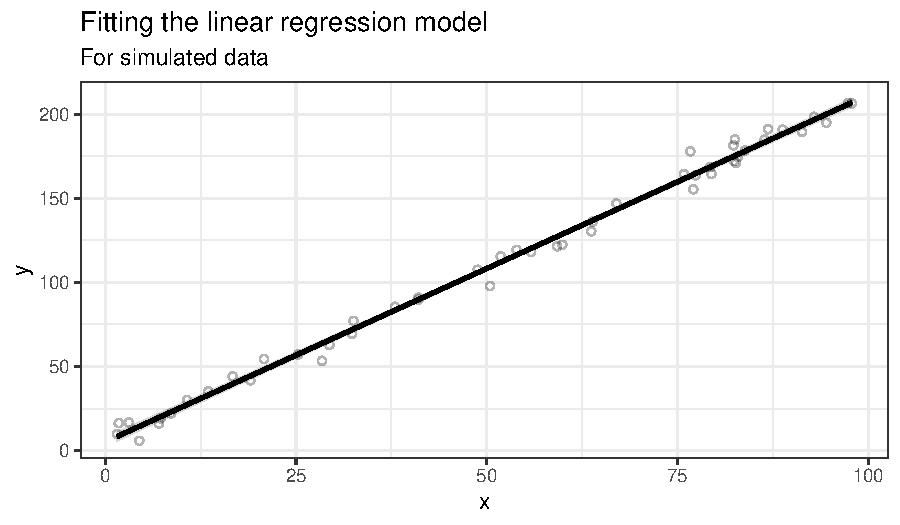
\includegraphics[width=\maxwidth]{figure/p4plot1-1} 
\end{knitrout}
\caption{Fitted model for \texttt{x} and \texttt{y}}
\label{p4plot1}
\end{center}
\end{figure}
It would appear that plot\ref{p4plot1} manages to approximate our data reasonably well. In order to verify its ability to explain the observation that we have, I suggest using $R^2$ value!


    \item Interpret the $R^2$ of the model.
\begin{knitrout}
\definecolor{shadecolor}{rgb}{0.969, 0.969, 0.969}\color{fgcolor}\begin{kframe}
\begin{alltt}
\hlkwd{paste}\hlstd{(}\hlstr{"Adjusted R-squared:"}\hlstd{, answer3}\hlopt{$}\hlstd{adj.r.squared)}
\end{alltt}
\begin{verbatim}
## [1] "Adjusted R-squared: 0.993695511395507"
\end{verbatim}
\end{kframe}
\end{knitrout}
This implies that 99\% of variance in data can be explained with the model that we've created! 
    \item Interpret the overall $F$ test of the model.
\begin{knitrout}
\definecolor{shadecolor}{rgb}{0.969, 0.969, 0.969}\color{fgcolor}\begin{kframe}
\begin{alltt}
\hlstd{answer3}\hlopt{$}\hlstd{fstatistic}
\end{alltt}
\begin{verbatim}
##   value   numdf   dendf 
## 7724.24    1.00   48.00
\end{verbatim}
\end{kframe}
\end{knitrout}
We have an incredibly high F-statistic which implies that our model has great predictive capability. Moreover, F-statistic shows (with $p<0.0001$) that our model provided us with the statistically significant results!

    \item Interpret the coefficients of the model; are they what you would expect?
They're exactly what I expected them to be. The intercept begins at 5.2, which is approximately the first data point in our dataset. Then, with each additional value of x, the value of y increases by 2.06. It seems to approximate the data rather well!

    \item Now, let's add a bad datapoint to the data.
\begin{knitrout}
\definecolor{shadecolor}{rgb}{0.969, 0.969, 0.969}\color{fgcolor}\begin{kframe}
\begin{alltt}
\hlstd{ggdat} \hlkwb{<-} \hlkwd{rbind}\hlstd{(ggdat,}     \hlcom{# original data}
               \hlkwd{c}\hlstd{(}\hlnum{100}\hlstd{,}\hlnum{25}\hlstd{))} \hlcom{# bad observation}
\end{alltt}
\end{kframe}
\end{knitrout}
  \begin{enumerate}
    \item Briefly summarize how adding this data point affects parts (a)-(g).
    Before giving any assessments, I would rather check with BFFITs if the added observation is an outlier.
\begin{knitrout}
\definecolor{shadecolor}{rgb}{0.969, 0.969, 0.969}\color{fgcolor}\begin{kframe}
\begin{alltt}
\hlstd{four.model}\hlkwb{<-}\hlkwd{lm}\hlstd{(y}\hlopt{~}\hlstd{x,} \hlkwc{data}\hlstd{=ggdat)}
\end{alltt}
\end{kframe}
\end{knitrout}
  
\begin{figure}[H]
\begin{center}
\begin{knitrout}
\definecolor{shadecolor}{rgb}{0.969, 0.969, 0.969}\color{fgcolor}\begin{kframe}
\begin{alltt}
\hlkwd{plotInfluence}\hlstd{(four.model)}
\end{alltt}
\end{kframe}
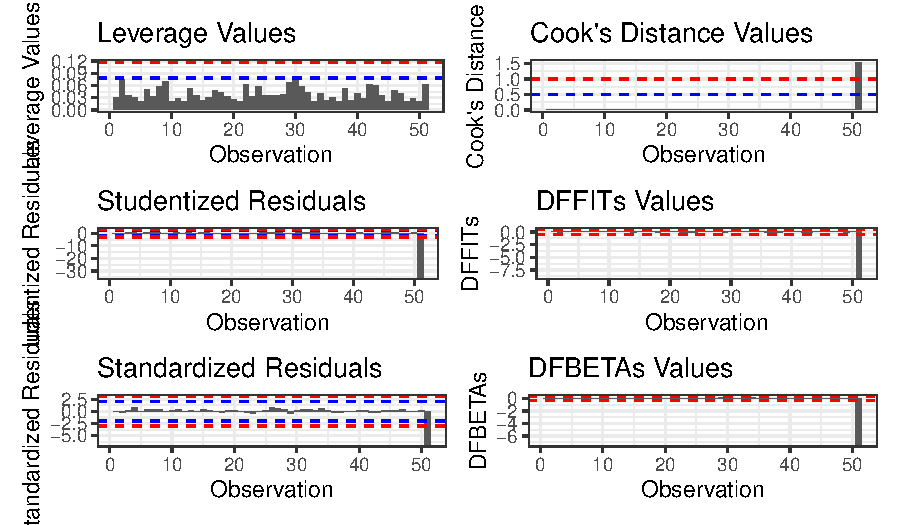
\includegraphics[width=\maxwidth]{figure/p4plot3-1} 
\end{knitrout}
\caption{Plots for asessing the influence of outliers on the linear regression model}
\label{p4plot3}
\end{center}
\end{figure}
Based on both Cook's Distance values and DFFITs values, we have a massive outlier that has an oversized influence on our regression model, compared to the previous datapoints. Therefore, it would be highly advisable to come up with a way to deal with it.
  
  
    \item Add the resulting regression line to the plot in part (d) in blue.
\begin{knitrout}
\definecolor{shadecolor}{rgb}{0.969, 0.969, 0.969}\color{fgcolor}\begin{kframe}
\begin{alltt}
\hlcom{#5.2+(2.06*x)}
\hlcom{#10.742+(1.891*x)}
\hlstd{ggdat.final} \hlkwb{<-} \hlstd{ggdat} \hlopt
  \hlkwd{mutate}\hlstd{(}\hlkwc{beforeAdding} \hlstd{=} \hlnum{5.2}\hlopt{+}\hlstd{(}\hlnum{2.06}\hlopt{*}\hlstd{x),}
     \hlkwc{afterAdding} \hlstd{=} \hlnum{10.742}\hlopt{+}\hlstd{(}\hlnum{1.891}\hlopt{*}\hlstd{x))}\hlopt
  \hlkwd{pivot_longer}\hlstd{(}\hlkwc{cols}\hlstd{=}\hlkwd{ends_with}\hlstd{(}\hlstr{"Adding"}\hlstd{),}
           \hlkwc{names_to}\hlstd{=}\hlstr{"Plot"}\hlstd{,}
           \hlkwc{values_to}\hlstd{=}\hlstr{"Pred"}\hlstd{)}
\end{alltt}
\end{kframe}
\end{knitrout}

\begin{figure}[H]
\begin{center}
\begin{knitrout}
\definecolor{shadecolor}{rgb}{0.969, 0.969, 0.969}\color{fgcolor}\begin{kframe}
\begin{alltt}
\hlkwd{ggplot}\hlstd{(ggdat.final,} \hlkwd{aes}\hlstd{(}\hlkwc{x}\hlstd{=x,} \hlkwc{y}\hlstd{=Pred))}\hlopt{+}
  \hlkwd{geom_smooth}\hlstd{(}\hlkwd{aes}\hlstd{(}\hlkwc{color}\hlstd{=Plot),}
              \hlkwc{method}\hlstd{=}\hlstr{"lm"}\hlstd{,}
              \hlkwc{formula}\hlstd{=y}\hlopt{~}\hlstd{x)}\hlopt{+}
  \hlkwd{geom_point}\hlstd{(}\hlkwd{aes}\hlstd{(}\hlkwc{y}\hlstd{=y),} \hlkwc{shape}\hlstd{=}\hlnum{1}\hlstd{,}
             \hlkwc{alpha}\hlstd{=}\hlnum{.3}\hlstd{)}\hlopt{+}
  \hlkwd{scale_color_manual}\hlstd{(}\hlkwc{values}\hlstd{=}\hlkwd{c}\hlstd{(}\hlstr{"black"}\hlstd{,} \hlstr{"blue"}\hlstd{),}
                     \hlkwc{label}\hlstd{=}\hlkwd{c}\hlstd{(}\hlstr{"After"}\hlstd{,}
                             \hlstr{"Before"}\hlstd{))}\hlopt{+}
  \hlkwd{labs}\hlstd{(}\hlkwc{title}\hlstd{=}\hlstr{"Fitting the linear regression models"}\hlstd{,}
       \hlkwc{subtitle}\hlstd{=}\hlstr{"For simulated data with an outlier"}\hlstd{,}
       \hlkwc{color}\hlstd{=}\hlstr{"Adding an outlier"}\hlstd{,}
       \hlkwc{y}\hlstd{=}\hlstr{"y"}\hlstd{)}
\end{alltt}
\end{kframe}
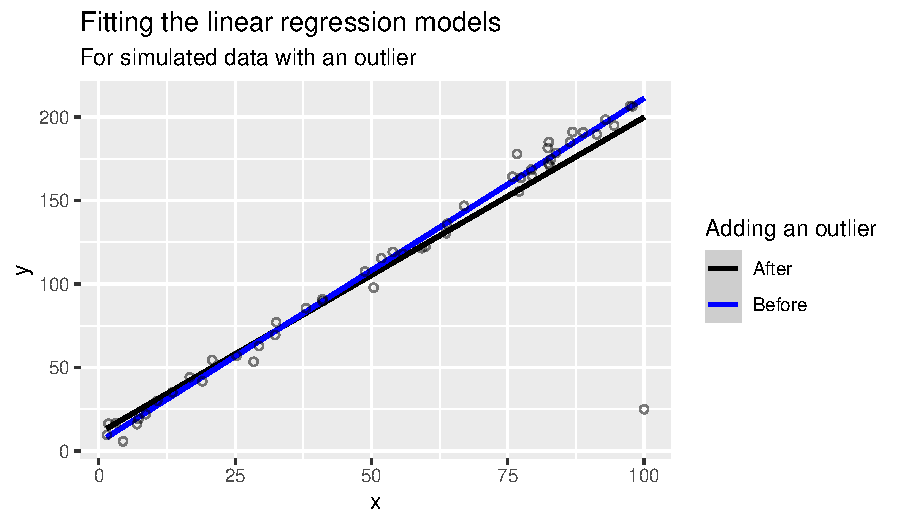
\includegraphics[width=\maxwidth]{figure/p4plot4-1} 
\end{knitrout}
\caption{Plot assessing the influence of an outlier on the linear regression model}
\label{p4plot4}
\end{center}
\end{figure}

It would appear that the outlier pulls our linear model down. Therefore, we can expect it to undervalue its predictions regarding our data. Before we go on to using various techniques of dealing with the bad observation, it's important to stress that in the scientific environment we ought to speak with the researchers first. Based on the field and the research context, it might be reasonable to leave those observations in the model.

    \item Refit this model using several robust techniques for dealing with the
    bad observation. Create a plot that summarizes all the approaches taken, and 
    use a metric to select the best model.

The first model we approach we are going to use is iteratively reweighted least squares.
\begin{knitrout}
\definecolor{shadecolor}{rgb}{0.969, 0.969, 0.969}\color{fgcolor}\begin{kframe}
\begin{alltt}
\hlkwd{library}\hlstd{(MASS)}
\hlkwd{library}\hlstd{(sfsmisc)}
\hlcom{#Hubert}
\hlcom{#6.0391 + (2.0421 * x) + e}
\hlstd{mod.hubert} \hlkwb{<-} \hlkwd{rlm}\hlstd{(y} \hlopt{~} \hlstd{x,} \hlkwc{data}\hlstd{=ggdat,}
                  \hlkwc{psi}\hlstd{=psi.huber)}
\hlkwd{summary}\hlstd{(mod.hubert)}
\end{alltt}
\begin{verbatim}
## 
## Call: rlm(formula = y ~ x, data = ggdat, psi = psi.huber)
## Residuals:
##       Min        1Q    Median        3Q       Max 
## -185.2474   -3.1410    0.5295    3.2745   15.3087 
## 
## Coefficients:
##             Value   Std. Error t value
## (Intercept)  6.0391  1.4224     4.2457
## x            2.0421  0.0228    89.7473
## 
## Residual standard error: 4.747 on 49 degrees of freedom
\end{verbatim}
\end{kframe}
\end{knitrout}
Result:\\
      \begin{align*}
      Huber=6.0391+(2.0421*x)+\epsilon\\
      \end{align*}

The second approach we're going to explore is the Bisquare iteratively reweighted least squares model.
\begin{knitrout}
\definecolor{shadecolor}{rgb}{0.969, 0.969, 0.969}\color{fgcolor}\begin{kframe}
\begin{alltt}
\hlcom{#5.7016 + (2.0504 * x)}
\hlstd{mod.bisquare}\hlkwb{<-}\hlkwd{rlm}\hlstd{(y} \hlopt{~} \hlstd{x,} \hlkwc{data}\hlstd{=ggdat,}
                  \hlkwc{psi}\hlstd{=psi.bisquare)}

\hlkwd{summary}\hlstd{(mod.bisquare)}
\end{alltt}
\begin{verbatim}
## 
## Call: rlm(formula = y ~ x, data = ggdat, psi = psi.bisquare)
## Residuals:
##      Min       1Q   Median       3Q      Max 
## -185.739   -3.265    0.056    3.033   15.011 
## 
## Coefficients:
##             Value   Std. Error t value
## (Intercept)  5.7016  1.4342     3.9755
## x            2.0504  0.0229    89.3722
## 
## Residual standard error: 4.607 on 49 degrees of freedom
\end{verbatim}
\begin{alltt}
\hlkwd{f.robftest}\hlstd{(mod.bisquare,} \hlkwc{var}\hlstd{=}\hlstr{"x"}\hlstd{)}
\end{alltt}
\begin{verbatim}
## 
## 	robust F-test (as if non-random weights)
## 
## data:  from rlm(formula = y ~ x, data = ggdat, psi = psi.bisquare)
## F = 7888.7, p-value < 2.2e-16
## alternative hypothesis: true x is not equal to 0
\end{verbatim}
\end{kframe}
\end{knitrout}
Result:\\
      \begin{align*}
      Bisquare=5.7016+(2.0504*x)+\epsilon\\
      \end{align*}

Since we are dealing with an outlier, it's also reasonable to use the quantile regression model. It's working with the median, so it won't be affected by the odd observation. 
\begin{knitrout}
\definecolor{shadecolor}{rgb}{0.969, 0.969, 0.969}\color{fgcolor}\begin{kframe}
\begin{alltt}
\hlkwd{library}\hlstd{(quantreg)}
\hlcom{#5.52 + (2.05*x)}
\hlstd{mod.quant} \hlkwb{<-} \hlkwd{rq}\hlstd{(y}\hlopt{~}\hlstd{x,} \hlkwc{data}\hlstd{=ggdat)}
\hlkwd{summary}\hlstd{(mod.quant,} \hlkwc{se} \hlstd{=} \hlstr{"ker"}\hlstd{)}
\end{alltt}
\begin{verbatim}
## 
## Call: rq(formula = y ~ x, data = ggdat)
## 
## tau: [1] 0.5
## 
## Coefficients:
##             Value    Std. Error t value  Pr(>|t|)
## (Intercept)  5.52886  2.88708    1.91504  0.06133
## x            2.05271  0.04751   43.20164  0.00000
\end{verbatim}
\end{kframe}
\end{knitrout}
Result:\\
\begin{align*}
      Quantile=5.52+(2.05*x)+\epsilon\\
      \end{align*}

Finally, let's compare the results we've got! 
\begin{knitrout}
\definecolor{shadecolor}{rgb}{0.969, 0.969, 0.969}\color{fgcolor}\begin{kframe}
\begin{alltt}
\hlcom{#6.0391 + (2.0421 * x) — Huber}
\hlcom{#5.7016 + (2.0504 * x) — Bisquare}
\hlcom{#5.52 + (2.05*x) — Quantile}

\hlstd{ggdat.compare} \hlkwb{<-} \hlstd{ggdat} \hlopt
  \hlkwd{mutate}\hlstd{(}\hlkwc{original_reg} \hlstd{=} \hlnum{5.2}\hlopt{+}\hlstd{(}\hlnum{2.06}\hlopt{*}\hlstd{x),}
         \hlkwc{OLS_reg} \hlstd{=} \hlnum{10.742}\hlopt{+}\hlstd{(}\hlnum{1.891}\hlopt{*}\hlstd{x),}
         \hlkwc{Huber_reg} \hlstd{=} \hlnum{6.0391} \hlopt{+} \hlstd{(}\hlnum{2.0421} \hlopt{*} \hlstd{x),}
         \hlkwc{Bisquare_reg} \hlstd{=} \hlnum{5.7016} \hlopt{+} \hlstd{(}\hlnum{2.0504} \hlopt{*} \hlstd{x),}
         \hlkwc{Quantile_reg} \hlstd{=} \hlnum{5.52} \hlopt{+} \hlstd{(}\hlnum{2.05}\hlopt{*}\hlstd{x),}
         \hlkwc{Population_reg} \hlstd{=} \hlnum{3.5}\hlopt{+}\hlstd{(}\hlnum{2.1}\hlopt{*}\hlstd{x))}\hlopt
  \hlkwd{pivot_longer}\hlstd{(}\hlkwc{cols}\hlstd{=}\hlkwd{ends_with}\hlstd{(}\hlstr{"_reg"}\hlstd{),}
               \hlkwc{names_to}\hlstd{=}\hlstr{"Plot"}\hlstd{,}
               \hlkwc{values_to}\hlstd{=}\hlstr{"Pred"}\hlstd{)}
\end{alltt}
\end{kframe}
\end{knitrout}

\begin{figure}[H]
\begin{center}
\begin{knitrout}
\definecolor{shadecolor}{rgb}{0.969, 0.969, 0.969}\color{fgcolor}\begin{kframe}
\begin{alltt}
\hlkwd{ggplot}\hlstd{(ggdat.compare,} \hlkwd{aes}\hlstd{(}\hlkwc{x}\hlstd{=x,} \hlkwc{y}\hlstd{=Pred))}\hlopt{+}
  \hlkwd{geom_smooth}\hlstd{(}\hlkwd{aes}\hlstd{(}\hlkwc{color}\hlstd{=Plot),}
              \hlkwc{method}\hlstd{=}\hlstr{"lm"}\hlstd{,}
              \hlkwc{formula}\hlstd{=y}\hlopt{~}\hlstd{x)}\hlopt{+}
  \hlkwd{geom_point}\hlstd{(}\hlkwd{aes}\hlstd{(}\hlkwc{y}\hlstd{=y),} \hlkwc{shape}\hlstd{=}\hlnum{1}\hlstd{,}
             \hlkwc{alpha}\hlstd{=}\hlnum{.3}\hlstd{)}\hlopt{+}
  \hlkwd{scale_color_manual}\hlstd{(}\hlkwc{values}\hlstd{=}\hlkwd{c}\hlstd{(}\hlstr{"black"}\hlstd{,} \hlstr{"blue"}\hlstd{,} \hlstr{"green"}\hlstd{,} \hlstr{"red"}\hlstd{,} \hlstr{"yellow"}\hlstd{,} \hlstr{"purple"}\hlstd{),}
                     \hlkwc{labels}\hlstd{=}\hlkwd{c}\hlstd{(}\hlstr{"Bisquare"}\hlstd{,} \hlstr{"Huber"}\hlstd{,} \hlstr{"OLS"}\hlstd{,} \hlstr{"Before outlier"}\hlstd{,} \hlstr{"Population"}\hlstd{,}
                              \hlstr{"Quantile"}\hlstd{))}\hlopt{+}
  \hlkwd{labs}\hlstd{(}\hlkwc{title}\hlstd{=}\hlstr{"Fitting the linear regression models"}\hlstd{,}
       \hlkwc{subtitle}\hlstd{=}\hlstr{"For simulated data with an outlier"}\hlstd{,}
       \hlkwc{color}\hlstd{=}\hlstr{"Technique"}\hlstd{,}
       \hlkwc{y}\hlstd{=}\hlstr{"y"}\hlstd{)}
\end{alltt}
\end{kframe}
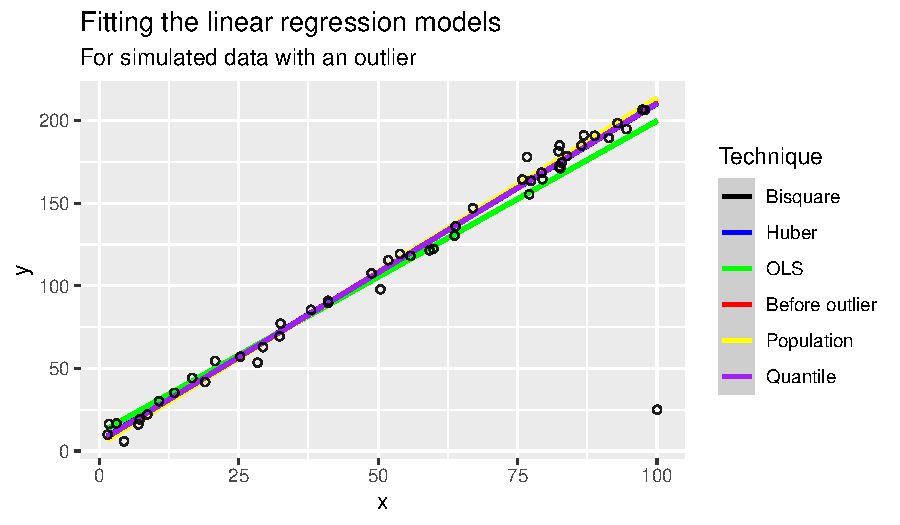
\includegraphics[width=\maxwidth]{figure/p4plot5-1} 
\end{knitrout}
\caption{Plot assessing the effect of robust techniques of dealing with bad observations}
\label{p4plot5}
\end{center}
\end{figure}

It would appear that most of the robust models that we've built essentially overlap with each other. I suggest that we can use root mean squared error to assess the model that fits data the most! Based on the visual inspection alone, I suggest that we can drop the OLS model, since it's too influenced by the outlier.
\begin{knitrout}
\definecolor{shadecolor}{rgb}{0.969, 0.969, 0.969}\color{fgcolor}\begin{kframe}
\begin{alltt}
\hlkwd{library}\hlstd{(Metrics)}

\hlkwd{rmse}\hlstd{(ggdat}\hlopt{$}\hlstd{y,} \hlkwd{predict}\hlstd{(mod.quant))}
\end{alltt}
\begin{verbatim}
## [1] 26.49428
\end{verbatim}
\begin{alltt}
\hlkwd{rmse}\hlstd{(ggdat}\hlopt{$}\hlstd{y,} \hlkwd{predict}\hlstd{(mod.hubert))}
\end{alltt}
\begin{verbatim}
## [1] 26.42363
\end{verbatim}
\begin{alltt}
\hlkwd{rmse}\hlstd{(ggdat}\hlopt{$}\hlstd{y,} \hlkwd{predict}\hlstd{(mod.bisquare))}
\end{alltt}
\begin{verbatim}
## [1] 26.48649
\end{verbatim}
\end{kframe}
\end{knitrout}

It would appear that Huber's IRWLS gives back the best results, so I suggest that we should use this model to predict the values. However, it's still important to stress the point that I've made earlier: before making any decisions, it's highly advisable to talk to the research partners to clarify their opinion on it. We might not have to even adjust our linear regression model! \\Communication is the key!\\Thank you for this semester, it was so much fun!

  \end{enumerate}
  \end{enumerate}
%%%%%%%%%%%%%%%%%%%%%%%%%%%%%%%%%%%%%%%%%%%%%%%%%%%%%%%%%%%%%%%%%%%%%%%%%%%%%%%
%%%%%%%%%%%%%%%%%%%%%%%%%%%%%%%%%%%%%%%%%%%%%%%%%%%%%%%%%%%%%%%%%%%%%%%%%%%%%%%
% End File
%%%%%%%%%%%%%%%%%%%%%%%%%%%%%%%%%%%%%%%%%%%%%%%%%%%%%%%%%%%%%%%%%%%%%%%%%%%%%%%
%%%%%%%%%%%%%%%%%%%%%%%%%%%%%%%%%%%%%%%%%%%%%%%%%%%%%%%%%%%%%%%%%%%%%%%%%%%%%%%
\end{enumerate}
\newpage
\bibliography{bib}
\end{document}
